\chapter{Knowledge Extraction from Deep Learning Models}
\label{chap:kbsextractiondl}
%ENLAZAR ESTO CON LOS PRINCIPIOS DE EXPLICABILIDAD DE PHILLIPS ET AL..
This chapter \footnote{Elvira Amador-Domínguez, Emilio Serrano, & Daniel Manrique (2021). A hierarchical multi-agent architecture (MAS) based on virtual identities to explain black-box personalization policies. Expert Syst. Appl., 186, 115731. doi:10.1016/j.eswa.2021.115731} showcases the extraction of knowledge from DL Models. Section \ref{6_sec:kbs_extra_dl_method} provides an overview on the design parameters of KBS extraction from DL models. Two instances of the proposed design are introduced in this chapter. The first instance focuses on \textit{black-box hyperpersonalization models} (BBHOS), DL models devised for user content personalization. Section \ref{6_sec:mas_bbhos_general} introduces this scenario, where a multi-agent system extracts behavioral patterns from the BBHOS. The MAS system is presented in Section \ref{6_sec:subsec:mas_description}, providing an example of its use in Section \ref{6_sec:subsec:case_study}. Section \ref{6_sec:subsec:mas_design_compliance} assesses the compliance of the proposed instance of the model with respect to the general method. 

Section \ref{6_sec:geni_main} outlines the second of the extraction instances. In this scenario, an explainability framework for extracting insights on the inference process of KGE models is presented. The proposed framework, GEnI, is described in Section \ref{6_sec:subsec:geni}. Sections \ref{6_sec:subsec:geni_evaluation} and \ref{6_sec:subsec:geni_results} depict the evaluation and analysis of the framework results, respectively. The compliance of the instance with respect to the general design parameters is portrayed in Section \ref{6_sec:subsec:geni_design_compliance}. Section \ref{6_sec:summary} summarizes the content of the chapter.


\section{Knowledge Extraction from Deep Learning Models}\label{6_sec:kbs_extra_dl_method}
In this context, the DL model acts as a passive element, from which the KBS is extracted by means of a middleware model. Method design parameters for KBS extraction from DL models are depicted in Figure \ref{fig:kbs_extra_dl_overview}.
\begin{figure}[t]
    \centering
    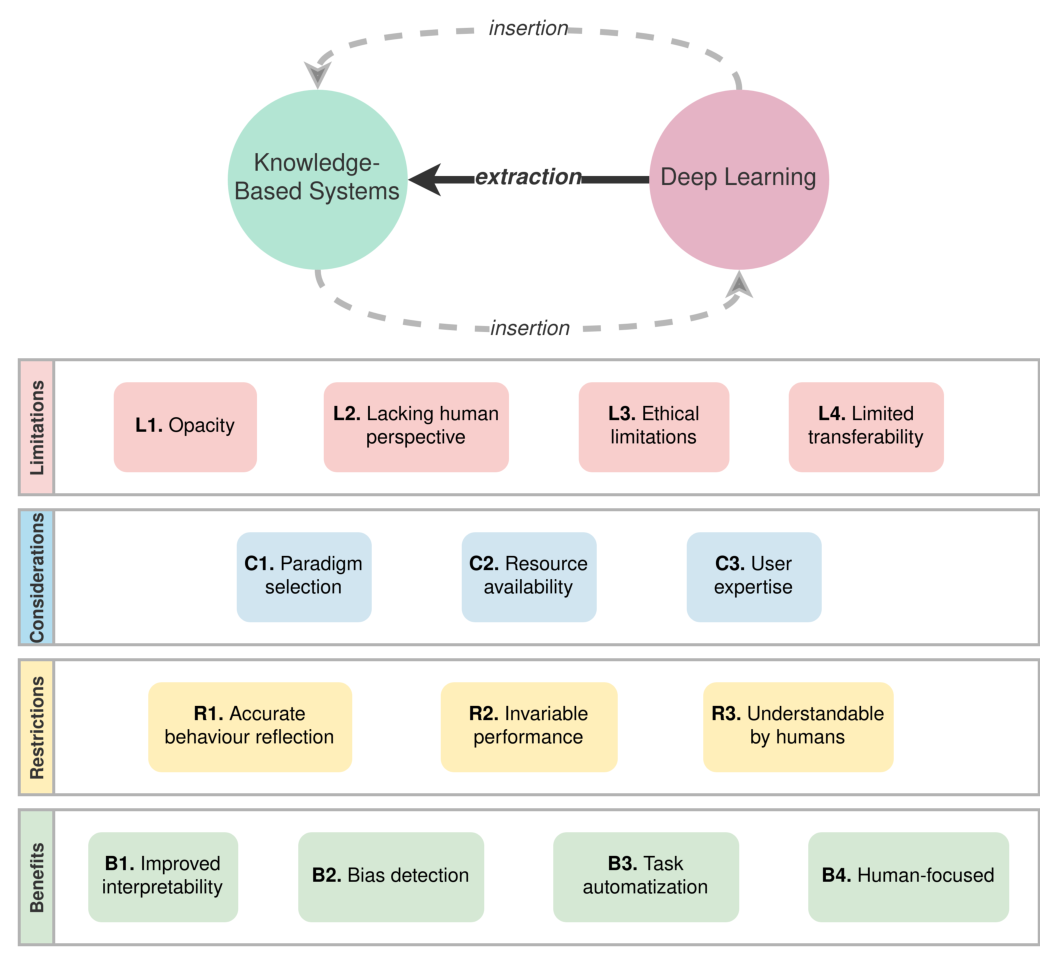
\includegraphics[width=\linewidth]{6_kbsextractiondl/figures/K_extraction_DL.eps}
    \caption{Overview on the Extraction of Knowledge-Based Systems from Deep Learning Models}
    \label{fig:kbs_extra_dl_overview}
\end{figure}

\paragraph{Limitations}
\begin{enumerate} [start=1,label={\bfseries L\arabic*.}]
    \item \textbf{Opacity.} \label{kbsextradl_L_opacity} As outlined in the limitations of KBS insertion in DL (Section \ref{4_sec:methodology_kbs_intro_dl}, \ref{kbsintrodl_L_opacity}), opacity is one of the main drawbacks of DL models. While some recent efforts aim to provide an insight on the inference process followed by a DL model to generate a certain output from a given input, these insights are only approximated. Therefore, explainations can reliably capture the behavior of the DL model, but it cannot be fully ascertain that they are an accurate depiction of the DL model's internal behavior.

    \item \textbf{Lacking human perspective.} \label{kbsextradl_L_human} DL models are devised to operate autonomously, without the need of human intervention. This phenomenon may be beneficial in some scenarios, but it may be detrimental when the user perspective is important. Such is the case of health related scenarios, where only expert users make final decisions and DL model predictions may not be fully trusted or justified. 
    
    \item \textbf{Ethical limitations.} \label{kbsextradl_L_ethical} DL models infer patterns entirely from training data. Therefore, the inferred patterns are not subject to any ethical considerations. This issue is particularly concerning, as biases within the data can lead to the inference of patterns that may be discriminating or exhibit some ethical concerns.
    
    \item \textbf{Limited transferability.}\label{kbsextradl_L_transferability} The lack of understanding on the internal behavior of DL models not only conditions its interactions with users, but also between models. This hinders the transferability of DL models, as it can not be ascertain beforehand how a model will behave on a different scenario.
\end{enumerate}

\paragraph{Considerations}
\begin{enumerate} [start=1,label={\bfseries C\arabic*.}]
    \item \textbf{Paradigm selection.} \label{kbsextradl_C_paradigm} KBS extraction from DL usually requires from one or more middleware models that perform the extraction and the conversion. Therefore, these models must be aligned with both the final KBS and the initial DL model. Moreover, if the KBS is devised as an explanatory mean for the DL model, it is also key to select a type of KBS that can accurately depict its behavior.
    
    \item \textbf{Resource availability.} \label{kbsextradl_C_resource} As evidenced in the previous interactions, the inclusion of DL models generally carries an additional computational cost. In this scenario, where the DL model is a passive element, its computational cost may not be as remarkable. However, the introduction of middleware models may increase the resource demand. Providing the involved models with sufficient computational resources is therefore essential.
    
    \item \textbf{User expertise.} \label{kbsextradl_C_user} In explainable AI, the focus shifts from the DL model to the user. Therefore, the extracted KBS should not only be aligned with the DL model, but also should be aligned with the final user. User expertise is an essential element in this scenario, as it conditions the KBS selection and behavior.
\end{enumerate}

\paragraph{Restrictions}
\begin{enumerate} [start=1,label={\bfseries R\arabic*.}]
    \item \textbf{Accurate behavior reflection.} \label{kbsextradl_R_behavior} If the KBS serves explainatory purposes, then it must be an accurate reflection of the behavior of the DL model. This implies that the KBS should not be considered a replacement for the DL model, nor improve its performance. The KBS must therefore imitate the behavior of the DL model.
    
    \item \textbf{Invariable performance.} \label{kbsextradl_R_performance} Whether the DL model serves as a source for KBS extraction, or acts as a black-box element to be explained, its performance must remain invariant and unaffected. This is particularly important regarding explainability, as modifications in the DL model may compromise their integrity, leading to inaccurate insights on its behavior. 
    
    \item \textbf{Human-understandable.} \label{kbsextradl_R_human} KBS are inherently symbolic, producing outputs that are human-readable. However, as denoted in \ref{kbsextradl_C_user}, the comprehensibility of the output does not only depend on the model, but on the expertise of the final user. Therefore, KBS must not only be readable, but comprehensible by humans.
\end{enumerate}

\paragraph{Benefits}
\begin{enumerate} [start=1,label={\bfseries B\arabic*.}]
    \item \textbf{Improved interpretability.}\label{kbsextradl_B_interpretability} Opacity is one of the main hardships regarding DL models (\ref{kbsextradl_L_opacity}). Gaining knowledge on the inference process of DL models increases the trust that users may have on the model (\ref{kbsextradl_L_human}). Moreover, it can serve as a scaffold for improving the transferability of the model (\ref{kbsextradl_L_transferability}).
    
    \item \textbf{Bias detection.}\label{kbsextradl_B_bias} Inference patterns learned by DL models are solely based on the input training data. Data is subject to errors and biases, which may cause the model to learn inferential patterns that, while accurate from a computational standpoint, may not be ethically correct (\ref{kbsextradl_L_ethical}). Being aware of the basis on which inference is performed may enable the detection of biases within the data, which can then be corrected.
    
    \item \textbf{Task automatization.}\label{kbsextradl_B_automatization} In addition to the explainability perspective, KBS extraction from DL can also be treated as a means for automatizing several tasks. In Section \ref{sec:sota_knowledge_extraction_dl}, ontology learning was presented as one of these cases, where ontologies were automatically mined. This approach can be taken for the automatization of different tasks, reducing the human effort required to perform them (\ref{kbsextradl_L_human}).
    
    \item \textbf{Human-focused.}\label{kbsextradl_B_human} DL models work virtually autonomously, minimizing the implication of users within the process. Making the models understandable by humans can increase the active implications of users within the learning process, not only increasing their trust but also enhancing the performance of the model from the inclusion of human knowledge (\ref{kbsextradl_L_human}). 
\end{enumerate}
%%HAY DOS CASOS DE USO. DAME TU FUERZA PEGASO QUE SE VIENE LA MADRE DE TODOS LOS INVENTS. 
\section{Behavioral Pattern Extraction from Black-Box Hyperpersonalization Models}\label{6_sec:mas_bbhos_general}

One of the main assets of DL models is their capacity to efficiently process vast amounts of heterogeneous data. Online marketing is one of the prominent areas where DL models are preferred, as they can ingest data from several data sources and generate accurate, fast responses. With the improvement of DL, marketing personalization policies have evolved from simpler statistical approaches, such as collaborative filtering, to the so-called \textit{hyper-personalization policies}. While classic personalization techniques group users by general, static traits (e.g., age, location), hyper-personalization policies incorporate dynamic and unique data about users (e.g., navigation data, sensor information). Hyper-personalization policies may improve user experience, but can raise some concerns, especially from the privacy protection perspective:

\paragraph{Opacity}
User data is the scaffold in which hyper-personalization policies are built. Some data is actively provided by the users from their publications in social media. However, a considerable amount of data still comes from mobile sensors and online activity, which is retrieved passively and unbeknownst to the user. Subsequently, when the user is faced with recommendations based solely on passively retrieved data, it can create a sense of rejection founded in a privacy invasion.

\paragraph{Limited adaptability} 
Hyper-personalization systems should be capable of automatically adapting to the user's needs. These changes may be detected from abrupt shifts in the user's data, causing the system to modify its behavior accordingly. However, there is generally a delay between the moment when the user context changes and when the system acts accordingly. Elevated delays may deter the user. Actively involving the user in the changing process may be a solution to this issue.

\paragraph{Lack of privacy}
Determining the optimal level of specificity for each user is a complex and challenging task. The accepted degree of personalization may vary between users. Thus, techniques that for some users may be acceptable, may be perceived as invasive for others. It is therefore crucial to ensure that the user feels comfortable with the level of personalization.

\paragraph{Absence of user input}
Users are at the core of hyper-personalization systems, whose goal is to accurately predict their needs. However, even though users are the most relevant component of these systems, their actual influence is minimal. Taking a hybrid approach, where the user actively participates in the personalization process, may not only create a sense of comfortableness, but enhance the behavior of the model.

A multi-agent system (MAS) based on virtual identities integrating user input is proposed to tackle the aforementioned issues. The MAS serves as an intermediary between the user and the \textit{black-box hyperpersonalization online systems} (BBHOS), thus hindering the recollection of passive data and improving user privacy. Additionally, the main goal of the proposed MAS is to analyze the behavior of BBHOS, extracting patterns on the responses of the system when faced with different user profiles. \textit{Generated virtual identities} (GVIDs) emulate the behavior of real-life users, each with a unique profile formed from a combination of predefined traits and dynamic information (e.g. contextual information, social media data). The MAS orchestrates the interactions between the GVIDs and the BBHOS, gathering a set of tailored responses for each GVID profile. Although BBHOS are opaque, general associative patterns between the profiles represented by each GVID and the responses generated for each of them can be inferred. These patterns can superficially explain the behavior of the BBHOS.

The knowledge extracted from these user profiling patterns can then be used for two different purposes: enhancing the privacy of the user and improving the relevance of the provided content. In the proposed system, the real user is masked by an agent, referred to as \textit{user virtualized identity} (UVID). The UVID acts as a surrogate, interacting with the BBHOS while simultaneously preventing the system from extracting information about the real user. While GVIDs have a passive role, being autonomously triggered and not interacting directly with the user, the UVID has an active role. Subsequently, the UVID is the only virtual identity able to perform certain transactions with the BBHOS. The proposed MAS adopts a hybrid solution, combining user interaction with autonomous behavior to achieve a balance between adaptability and user reliability. In addition to triggering certain transactions, the user input also determines the validity of the personalized content provided by the BBHOS.

\subsection{A Hierarchical Multi-Agent Architecture Based on Virtual Identities}\label{6_sec:subsec:mas_description}

Figure \ref{fig:overview_mas} showcases the proposed four-layered MAS. Each layer comprises a set of agents that perform a series of actions specific to each layer. Agents can communicate with other agents both from the same and adjacent layers. In addition to the MAS layers, a storage layer is included to store and manage the collected data. Layers can be grouped into two levels: autonomous and user-triggered. The autonomous level of the system aggregates the first two layers, which comprises those actions that execute without any user interaction and prepare the system for its subsequent use. The user-triggered level, associated with layers three and four, is reliant on the user to execute. 

\begin{figure}[t]
    \centering
    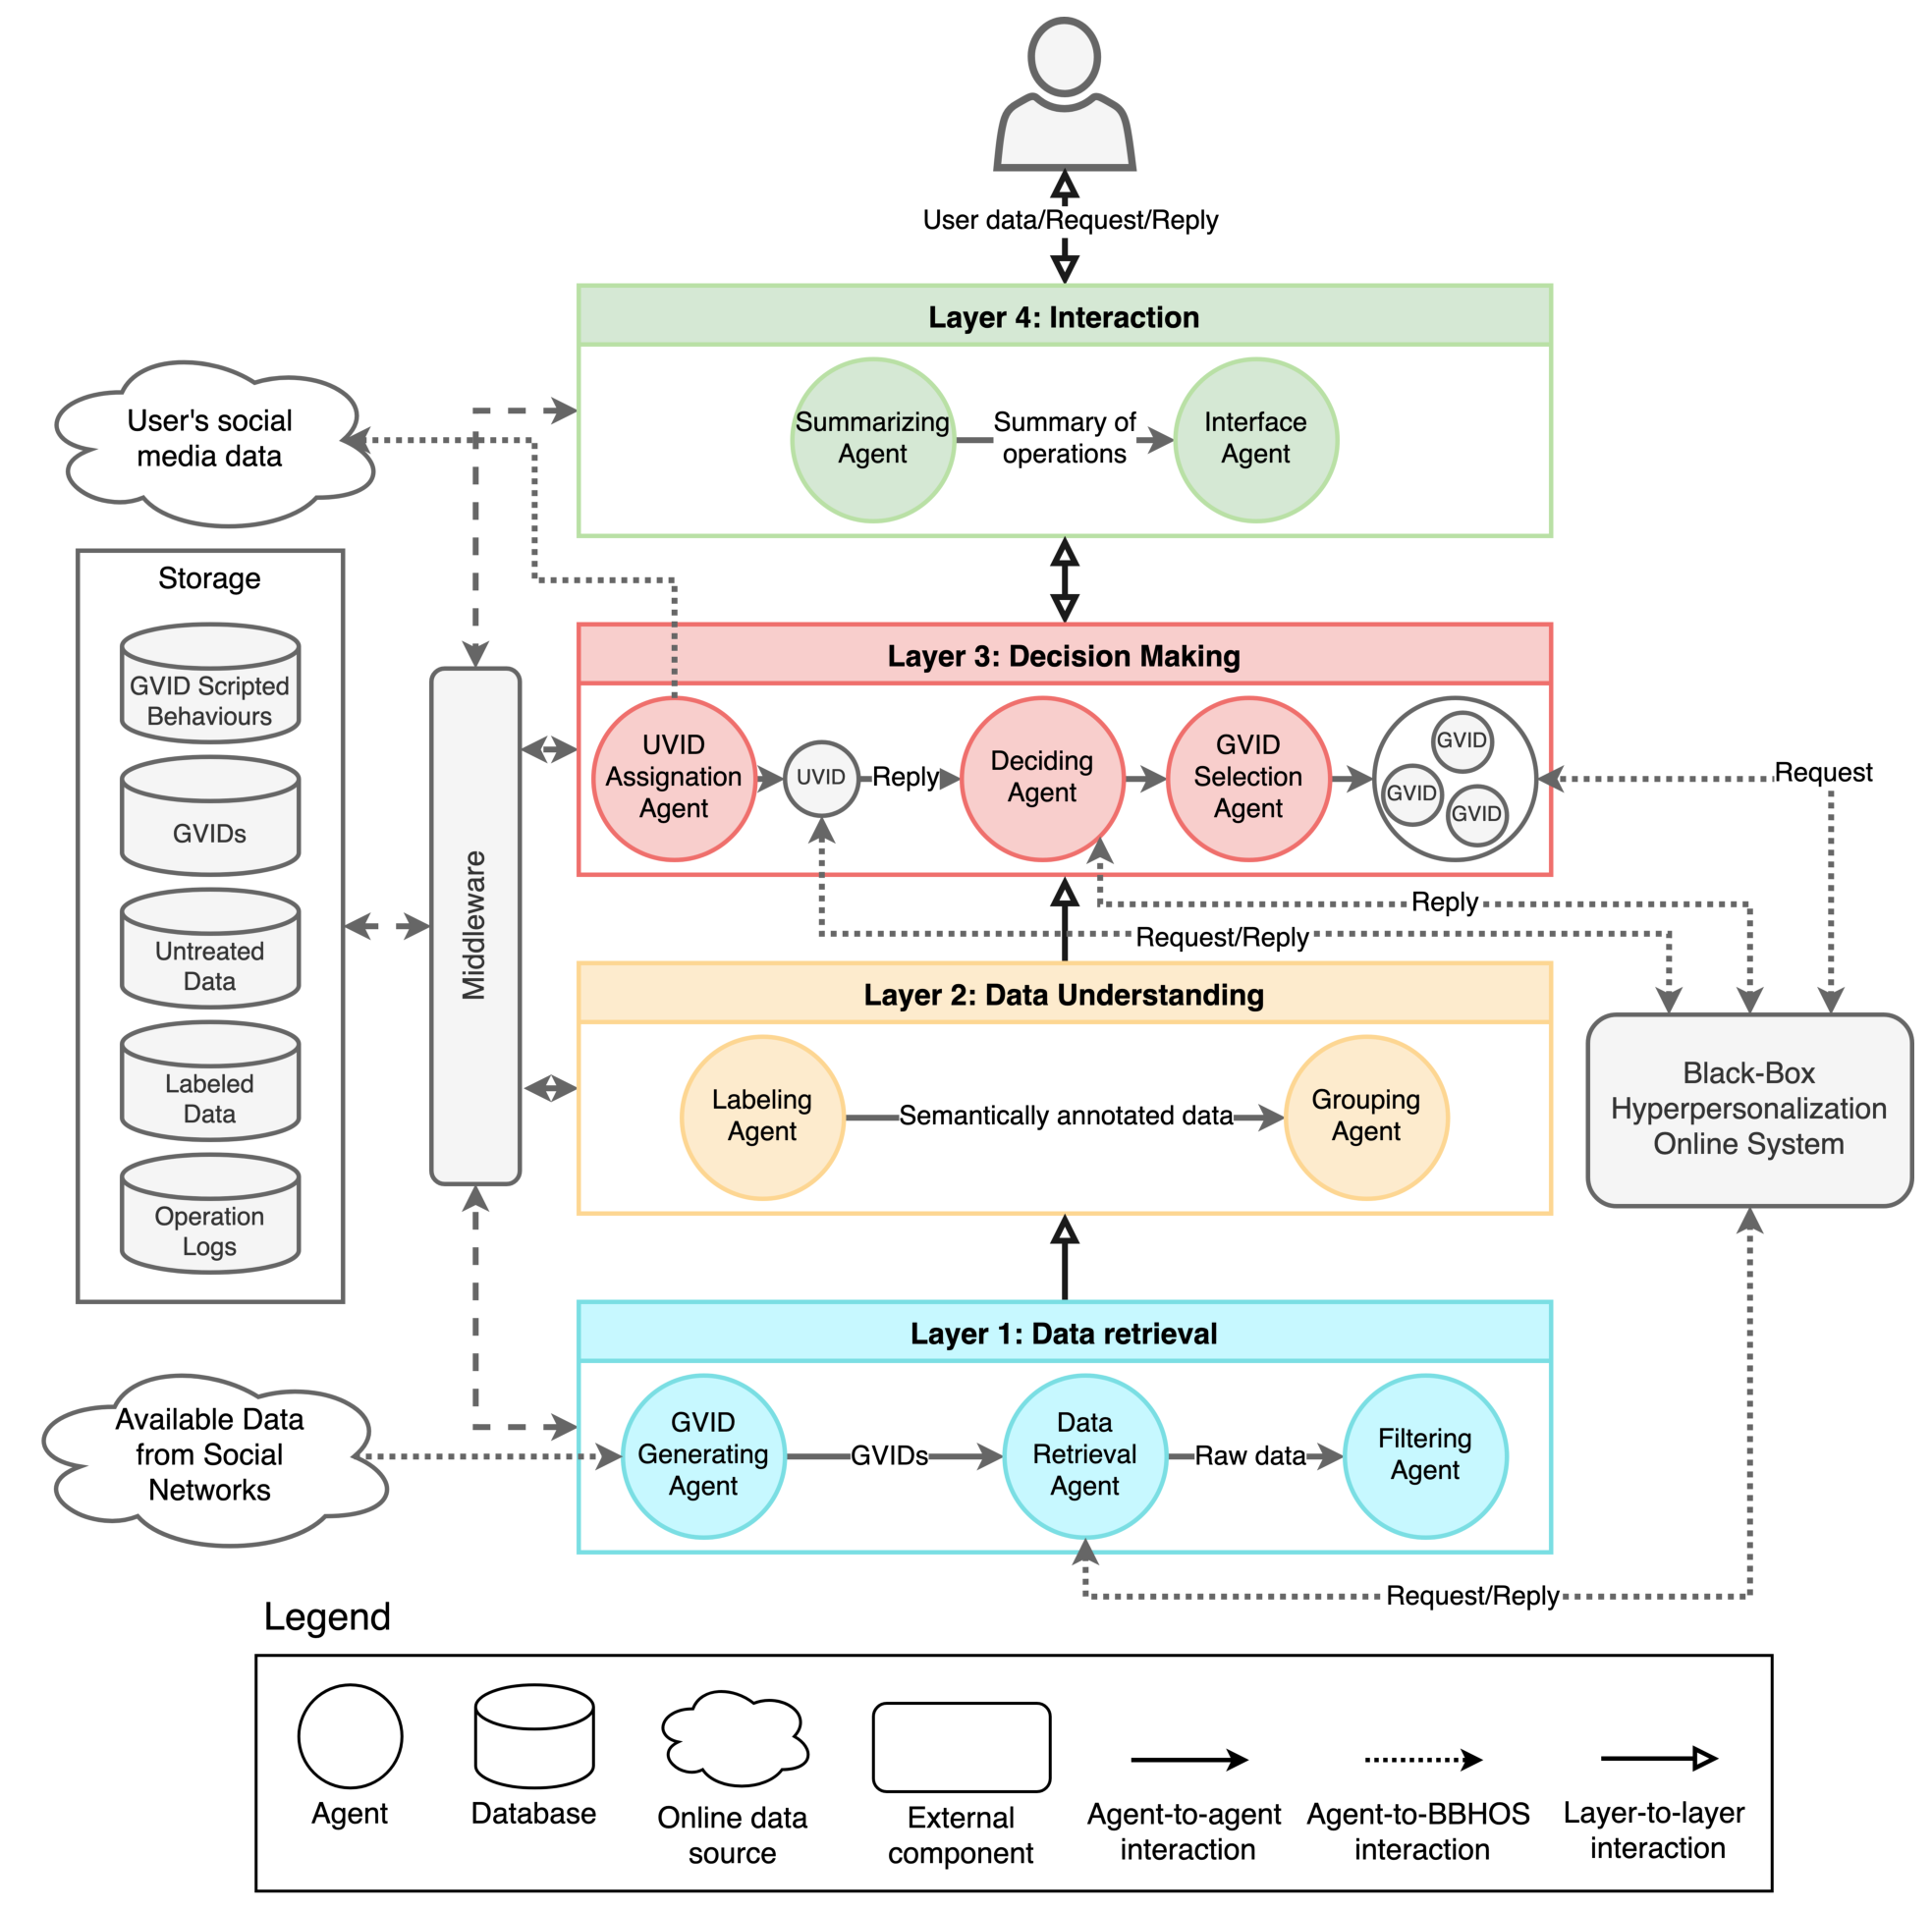
\includegraphics[width=.9\linewidth]{6_kbsextractiondl/figures/Overview_MAS.eps}
    \caption{Overview of the proposed hierarchical multi-agent system.}
    \label{fig:overview_mas}
\end{figure}

\subsubsection*{Layer 1: Data retrieval}
The first layer of the MAS comprises the operations related to the creation of GVIDs, as well as the BBHOS data extraction. This layer sets the purpose and goal of the system, selecting the BBHOS to study and the behavior of the GVIDs. Three agents can be identified in this layer:
\begin{itemize}
    \item \textit{GVID generating agent.} Two elements are considered by this agent to generate the GVIDs, providing them with unique features and enabling the realistic emulation of the behavior of real-life users. The first element are the core GVID features, which are stored in the system. These features include static treats such as gender, age, name, location, or interests. 
    
    Since static features are not enough to realistically emulate the behavior of a user, social media data is also scrapped to generate user profiles. This data is collected \textit{ad-hoc} from external sources and its not stored in the system. Natural Language Processing (NLP) techniques are used to analyze and extract relevant information from this data, such as topic modeling \citep{Alghamdi2015} or sentiment analysis \citep{sentimentanalysis}. Information such as preferences, opinions, or interests can be extracted from this data, which can then be added alongside the static traits of the GVIDs to generate more complex, human-like behaviors. GVIDs are stored, and subsequently used by the superior layers of the system. 
    
    \item \textit{Data retrieval agent.} GVIDs interact with the BBHOS by making requests and receiving responses, which are aligned with their features and behaviors. This agent orchestrates and supervises the interactions between the GVIDs and the services, collecting the data generated in the process. Data can have different different formats, according to the targetted BBHOS, ranging from plain text to video files. Collected data is stored for further analysis, as it can be used to redefine the static traits of the GVIDs.
    
    As BBHOS are online systems and are subject to network-related issues, which need to be corrected before transmitting the data to the next agent. Hence, this agent also performs operations such as duplicate or corrupted data removal. 
    
    \item \textit{Filtering agent.} This agent receives the interaction data between the GVIDs and the BBHOS, and classifies it according to its format (e.g., image, text, or audio). Filtering and homogenization operations are performed to extract relevant content from the received data and to facilitate the usage of data understanding processes. According to the data format, suitable filtering operations may be required, such as normalization or text preprocessing. This agent only considers formal aspects of the content.
\end{itemize}

\subsubsection*{Layer 2: Data understanding}
Data understanding processes are needed to extract knowledge from the outputs of the interactions between the GVIDs and the BBHOS. The second layer of the MAS deals with the procedures required for this task. General knowledge on the behavior of the BBHOS can be inferred from the analysis of the content fed to each particular profile (encoded on the GVIDs). Two agents comprise this layer:
\begin{itemize}
    \item \textit{Labelling agent.} This agent annotates, classifies, and extracts knowledge from the collected interaction data. Due to the heterogeneity amongst data types, suitable approaches are required to effectively extract knowledge from the unstructured data. Multi-label classification using Convolutional Neural Networks (CNNs) \citep{He2015DeepRL,CNNRNN} can be used for image treatment, detecting the elements included in an image. CNNs can also be used for audio and video classification \citep{HersheyCEGJMPPS16}. For further processing, audio can be transcribed \citep{speechrecognition} to enable text operations. 
    
    The majority of the responses generated by the BBHOS are textual, thus requiring a more profound analysis than the aforementioned data formats. Multiple NLP techniques can be considered to analyze textual data from distinct perspectives. Text classification techniques \citep{MIRONCZUK201836} may be suitable to categorize the retrieved content. Topic modelling \citep{pmlr-v15-nallapati11a,Alghamdi2015} enable finer-grained classification and content analysis. Additionally, document clustering, as well as text summarizing techniques \citep{Neto00documentclustering,YOUSEFIAZAR201793,Oikonomakou2005} can be used to simplify and group the data, facilitating its comprehension.
    
    The annotated data is then stored in the system. As most of the state-of-the-art approaches for the aforementioned tasks rely on deep learning models, periodical retrainings may be needed to keep the models updated.
    
    \item \textit{Grouping agent.} While BBHOS are opaque, associative patterns may be inferred based on the responses provided to each particular GVID. Furthermore, GVIDs can be grouped based on the similarity of their targeted responses. This agent establishes GVID aggregation based on this information, using a hierarchical approach ranging from specific to general. Therefore, heterogeneity between the lower level clusters is maintained, while converging into a single aggregation in the final top level. GVID aggregations are stored in the system.
\end{itemize}

\subsubsection*{Layer 3: Decision Making}
In this layer, the user's data input is collected, processed, and sent to the final interaction layer. While the previous two layers follow a forward-only criterion, where the data flows from inferior to superior layers, this layer has a bidirectional flow. This layer can therefore be considered the core element of the system, and its execution is triggered directly by the user. This layer comprises three agents:
\begin{itemize}
    \item \textit{UVID assignation agent.} This agent creates and deploys a virtual identity that represents the real user within the system, referred to as the \textit{User Virtual Identity} (UVID). The UVID serves as an intermediary between the BBHOS and the user, protecting the user from potential privacy invasions. Similarly to GVIDs, the static information provided about the user is complimented with available social media data, whose recollection must be approved by the user. Moreover, the UVID also encodes the user's specifications on the content, thus serving as a filter. 
    
    \item \textit{Deciding agent.} Once the UVID is deployed, it interacts with the BBHOS. If the retrieved content meets the user's specifications, the response is then transferred to the superior layer, where the user can approve it. If not approved, this agent passes this information to the \textit{GVID selection agent}, which querys the BBHOS generating a new set of responses. This agent is aware of the user's requirements and decides which, if any, of the returned responses are suitable. If there are no valid responses, this agent reenacts the query to the BBHOS to receive new responses. This process is iteratively performed until the user indicates the validity of the response, or until no GVID aggregations remain.
    
    This agent orchestrates the interactions between the GVIDs and the BBHOS and collects the information from the real user and distributes it to the following agent. The data generated by this agent is also stored for further analysis.
    
    \item \textit{GVID Selection Agent.} If the response received by the UVID does not satisfy the user requirements, new responses are required as shown in Figure \ref{fig:overview_mas}. A new GVID set is selected if the \textit{deciding agent} sends a negative response. Since a specific-to-general approach is considered, similar GVID aggregations are first selected. If the user professes a strong rejection on the previous BBHOS response, then the agent may select a polar opposite GVID set in the following iteration.
    
    The initial GVID set is selected according to the similarity between the UVID and the existing GVID sets. As GVIDs are arranged hierarchically, a nearest neighbour criterion can be used. Thus, the aggregation containing the most similar GVID to the UVID is selected in the first place.

    \begin{figure}[t]
        \centering
        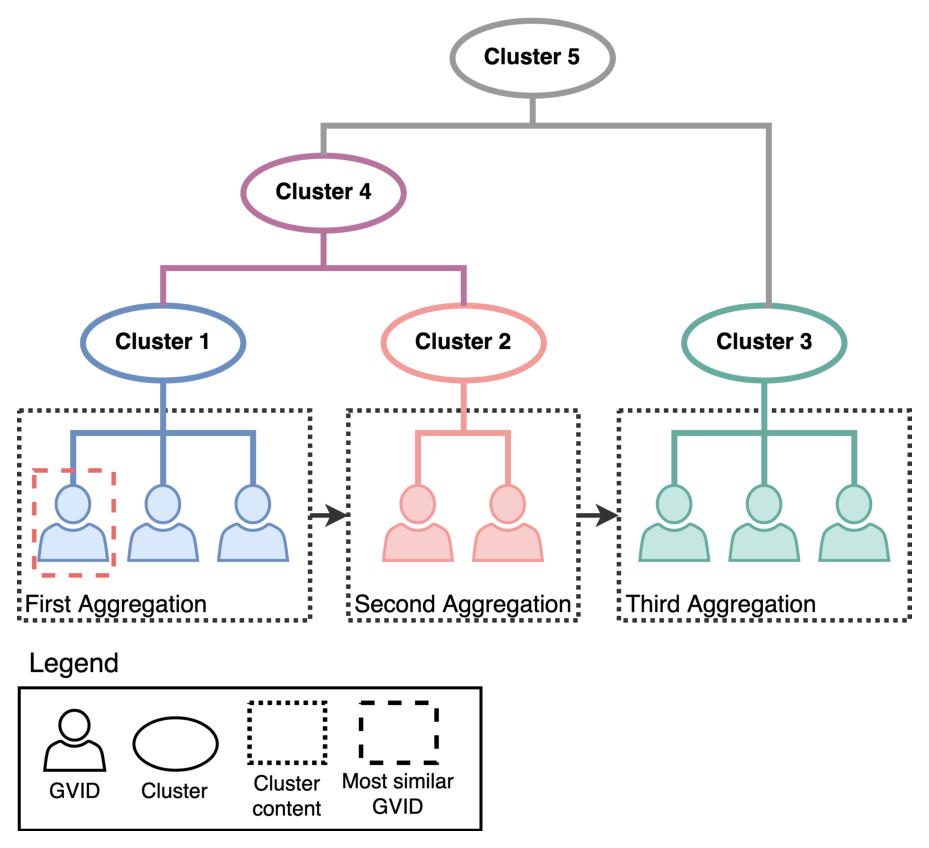
\includegraphics[width=.65\linewidth]{6_kbsextractiondl/figures/GVID_clusters.eps}
        \caption{Example of the GVID selection procedure.}
        \label{fig:gvid_selection}
    \end{figure}
    
    Figure \ref{fig:gvid_selection} depicts the general selection procedure. The GVID with the highest similarity to the UVID belongs to \textit{cluster 1}. Therefore, \textit{cluster 1} is selected as the initial GVID set. Then, the superior level of the hierarchy is explored (\textit{cluster 4}), which is composed of clusters 1 and 2. As \textit{cluster 1} has already been selected, \textit{cluster 2} would be selected as the next GVID aggregation. If the user does not express a strong disagreement with the provided responses, the system follows the specified hierarchical order to select the following aggregations.
\end{itemize}

\subsubsection*{Layer 4: Interaction}
Finally, an interaction layer is included to present the result of the operations performed in the inferior layers to the user. The data flow in this layer is also bidirectional, as the user not only receives, but introduces information in the system. User input is key to the system, as it conditions its behavior. The agents of this layer determine what and how the content is displayed to the user. They also collect input from the user and forward it to the inferior layers.

\begin{itemize}
    \item \textit{Summarizing agent.} To maintain the system's transparency, both the output and the log of the operations required for its generation are provided to the user. This agent extracts the logs of the iterations required by the \textit{deciding agent} to reach its final reply, and summarizes the most relevant information. Alongside the output, this agent generates a simple, user-readable record on which GVID received each response, as well as how many iterations were required. Thus, the real user can be conscious of whether the final response was obtained by the UVID or a different user profile (GVID).
    
    \item \textit{Interface agent.} User input is essential for the behavior of the system at its superior level. Appropriate mechanisms to interact with the user and correctly fulfill their requirements are needed. The communication with the user is established bidirectionally, implying that the system not only collects the user's input, but also generates an output that must be clear and readable. Therefore, this agent serves as a direct intermediary between the user and the system. The user's input is collected and transmitted to the lower layer for processing. Besides, this agent receives the output from the \textit{summarizing agent} containing the final BBHOS response and operation logs. This content is then displayed to the user in a simplified and visual format.
\end{itemize}

\subsubsection*{Storage units}
As depicted in Figure \ref{fig:overview_mas}, storage units serve as a sharing point for all MAS layers. The data generated during the system execution is heterogeneous, coming from different sources and in different formats. Five distinct databases are set to suit the different data types generated within the system:
\begin{itemize}
    \item \textit{GVID scripted behaviors.} Unique features are required to create a variety of user profiles to analyze the behavior of BBHOS. These features refer to mid-term information, such as interests or age, which remains static throughout the execution.
    
    \item \textit{Untreated data.} This unit stores data extracted from the interactions between the GVIDs and the BBHOS in the first execution stages. The responses obtained from the BBHOS can then be used to redefine the behavior of the GVIDs.
    
    \item \textit{Labeled data.} Once untreated data has been filtered, categorized, and annotated is stored in this database. This data can then be used to periodically retrain the models in the \textit{labeling agent} to keep the system updated. 
    
    \item \textit{GVIDs.} GVIDs are at the core of the system and used by multiple agents of the system across different layers. Therefore, it is critical to ensure their persistence and accessibility. As well as the single GVIDs generated in the first layer of the system, the aggregations obtained after performing hierarchical clustering is also stored within this unit. If there is a change in the GVIDs, a reaction to the \textit{GVID generating agent} is unchained, initiating the execution of the autonomous level of the MAS.
    
    \item \textit{Operation logs.} A log of the communications between the GVIDs and the selected BBHOS is saved. The data generated from these interactions enables the extraction of associative patterns that enable understanding over the BBHOS. These logs are generated in the third layer and used in the fourth for summarization.
\end{itemize}

Additionally, there is a \textit{middleware} between the databases and the agents that orchestrates and supervises the introduction and extraction of data from the different databases. The middleware also ensures data persistence and avoids concurrency issues.

\subsection{Data Flow}\label{6_sec:subsec:data_flow}

\begin{figure}[t]
    \centering
    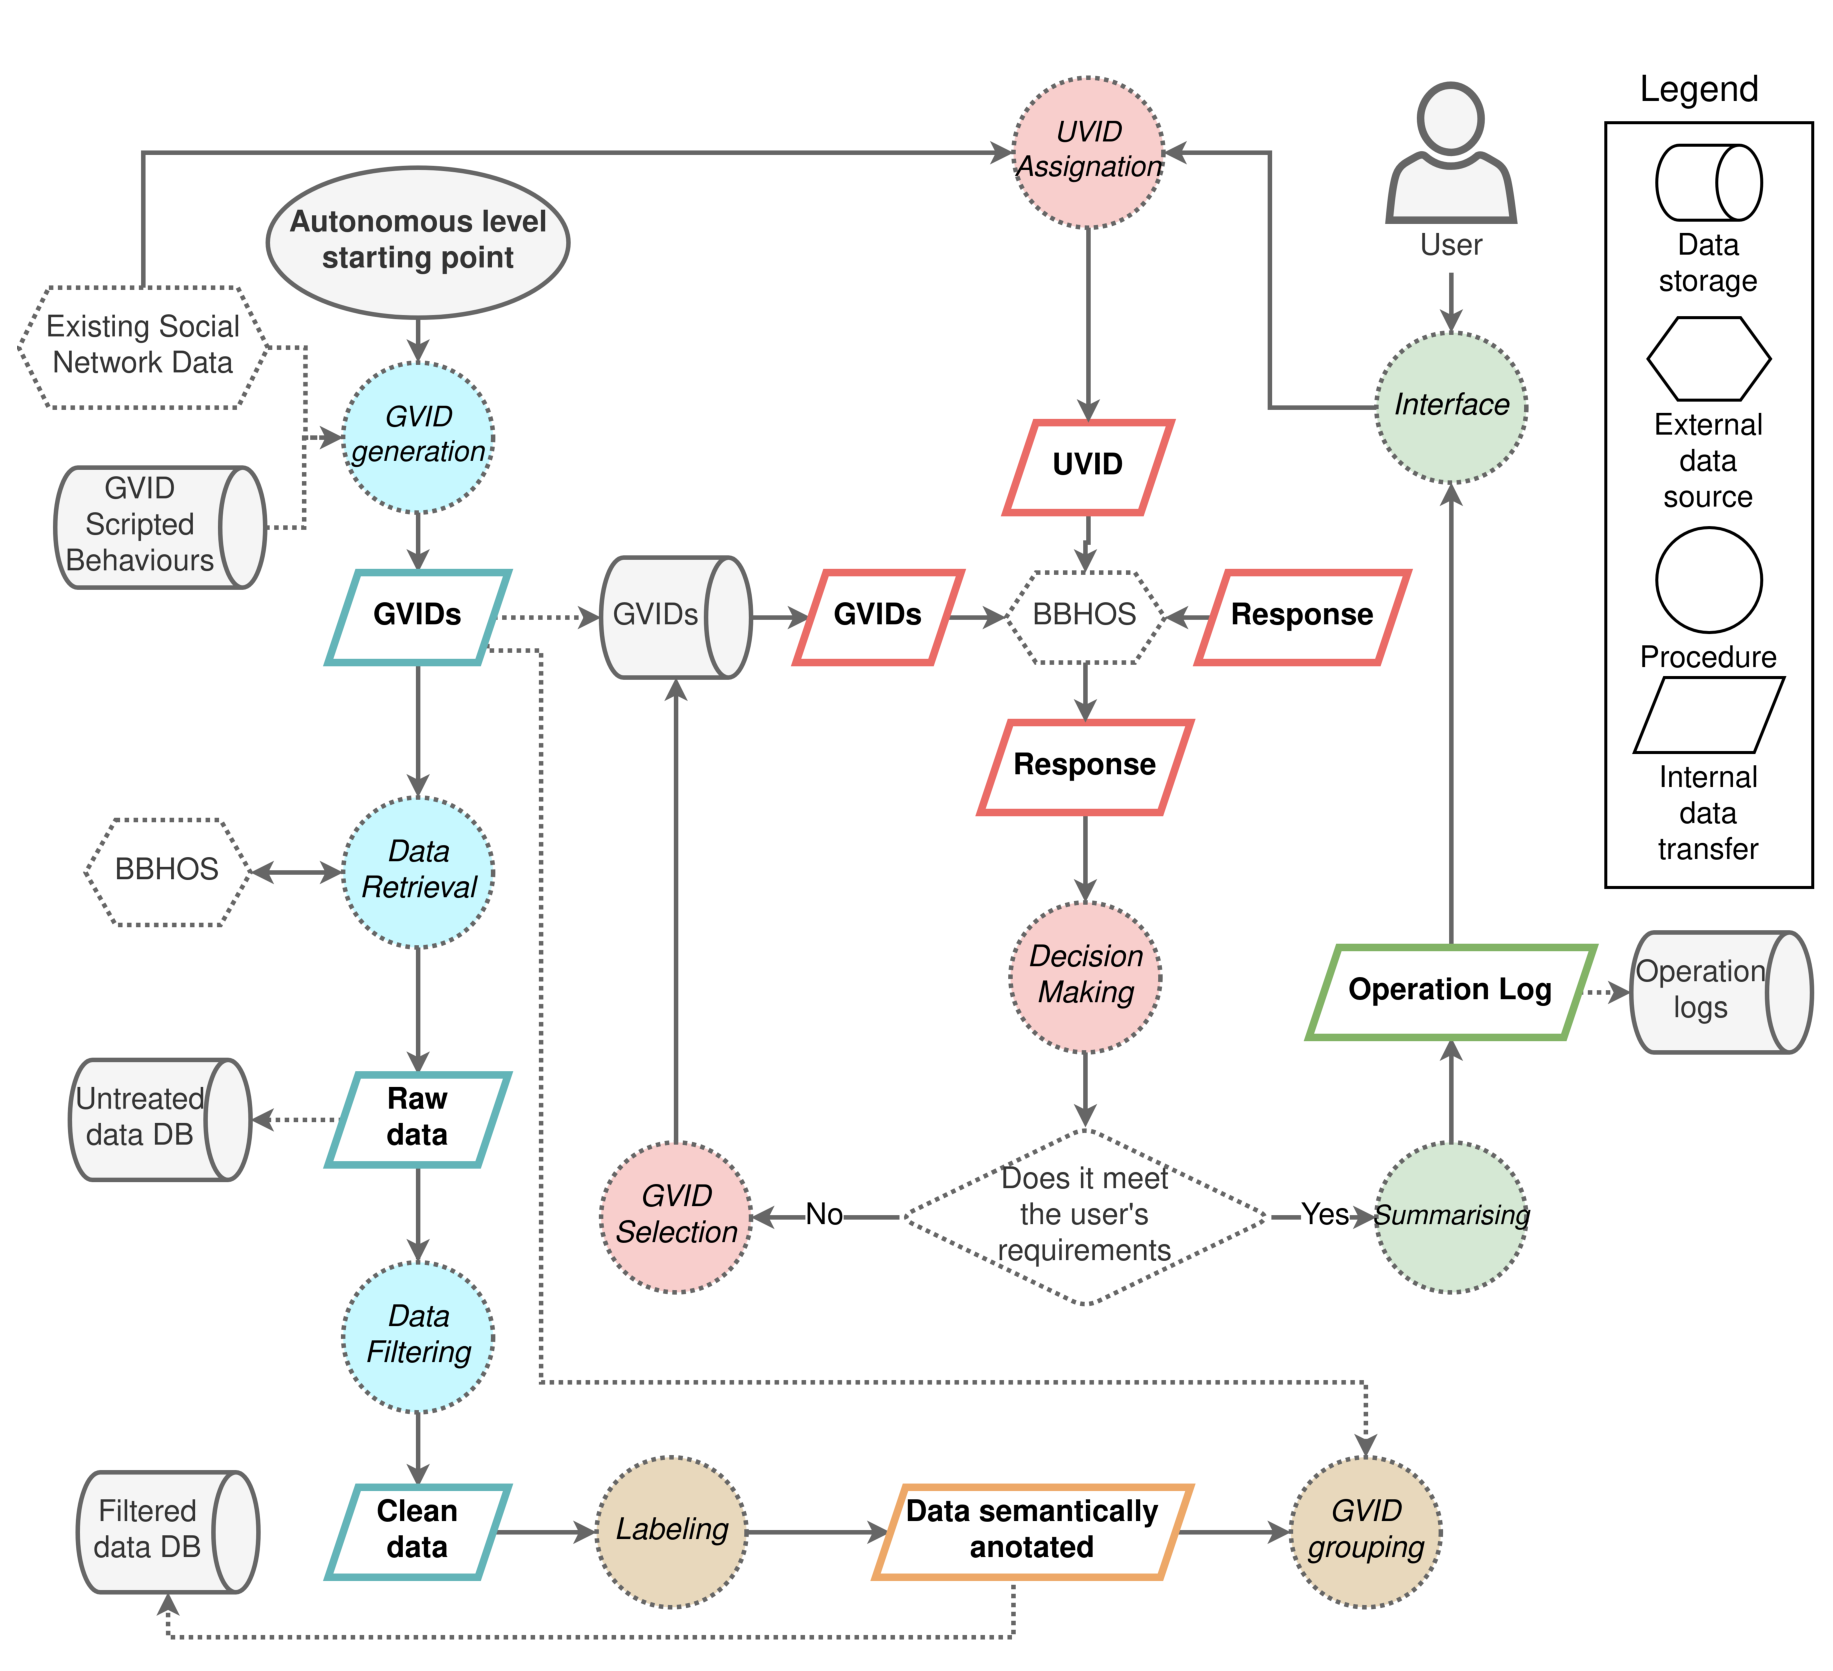
\includegraphics[width=\linewidth]{6_kbsextractiondl/figures/Data_flow.eps}
    \caption{Data flow of the proposed MAS. }
    \label{fig:data_flow_mas}
\end{figure}

Figure \ref{fig:data_flow_mas} depicts the data flow of the proposed MAS. Once the autonomous level of the system initiates, GVIDs are generated from a combination of scripted behaviors and existing social network data. The generated GVID set is then stored in the GVID database. GVIDs then interact with the BBHOS, receiving a set of responses in raw format, which are also stored for further analysis and GVID behavior correction. 

Response data at this stage remains untreated, containing both relevant and irrelevant information. This data is first classified according to its format into video, audio, image, and text to facilitate its annotation and analysis. Appropriate filtering and homogenization operations are performed on the data, according to its format. Images are resized and normalized, while markup and stopword removal is performed on textual data. Filtering and cleaning the data not only eases the annotation, but also considerably reduces its size. The models in the \textit{labeling agent} then annotate the filtered data and store it in its corresponding database. Hierarchical clustering is then performed to aggregate the GVIDs with respect to the content of their responses. GVID clusters are also stored in the GVID database.

The previous operations belong to the autonomous level and are subsequently executed without any user interaction. In the second level of the system, comprised by layers three and four, the user is the entry point, and its interaction with the system triggers its execution. The user accesses the system from the interface, specifying a set of goals and specifications. Then, the UVID is generated. The UVID then interacts with the BBHOS, receiving a targeted response. If this response meets the user's requirements, it is then summarized and forwarded to the user using the \textit{interface agent}. On the contrary, if the user rejects the response or it is not aligned to the specified requirements, a set of GVIDs are selected, repeating the same request over the BBHOS. Once the user agrees with a response, the user-triggered level of the system is suspended until further interaction.

\subsection{Case Study}\label{6_sec:subsec:case_study}


This Section presents a case study to illustrate the proposed architecture. This case study aims to provide a clearer and deeper insight on the interactions and data transfer between agents, giving a complete overview on the behavior of the system. 

\begin{figure}[t!]
    \centering
    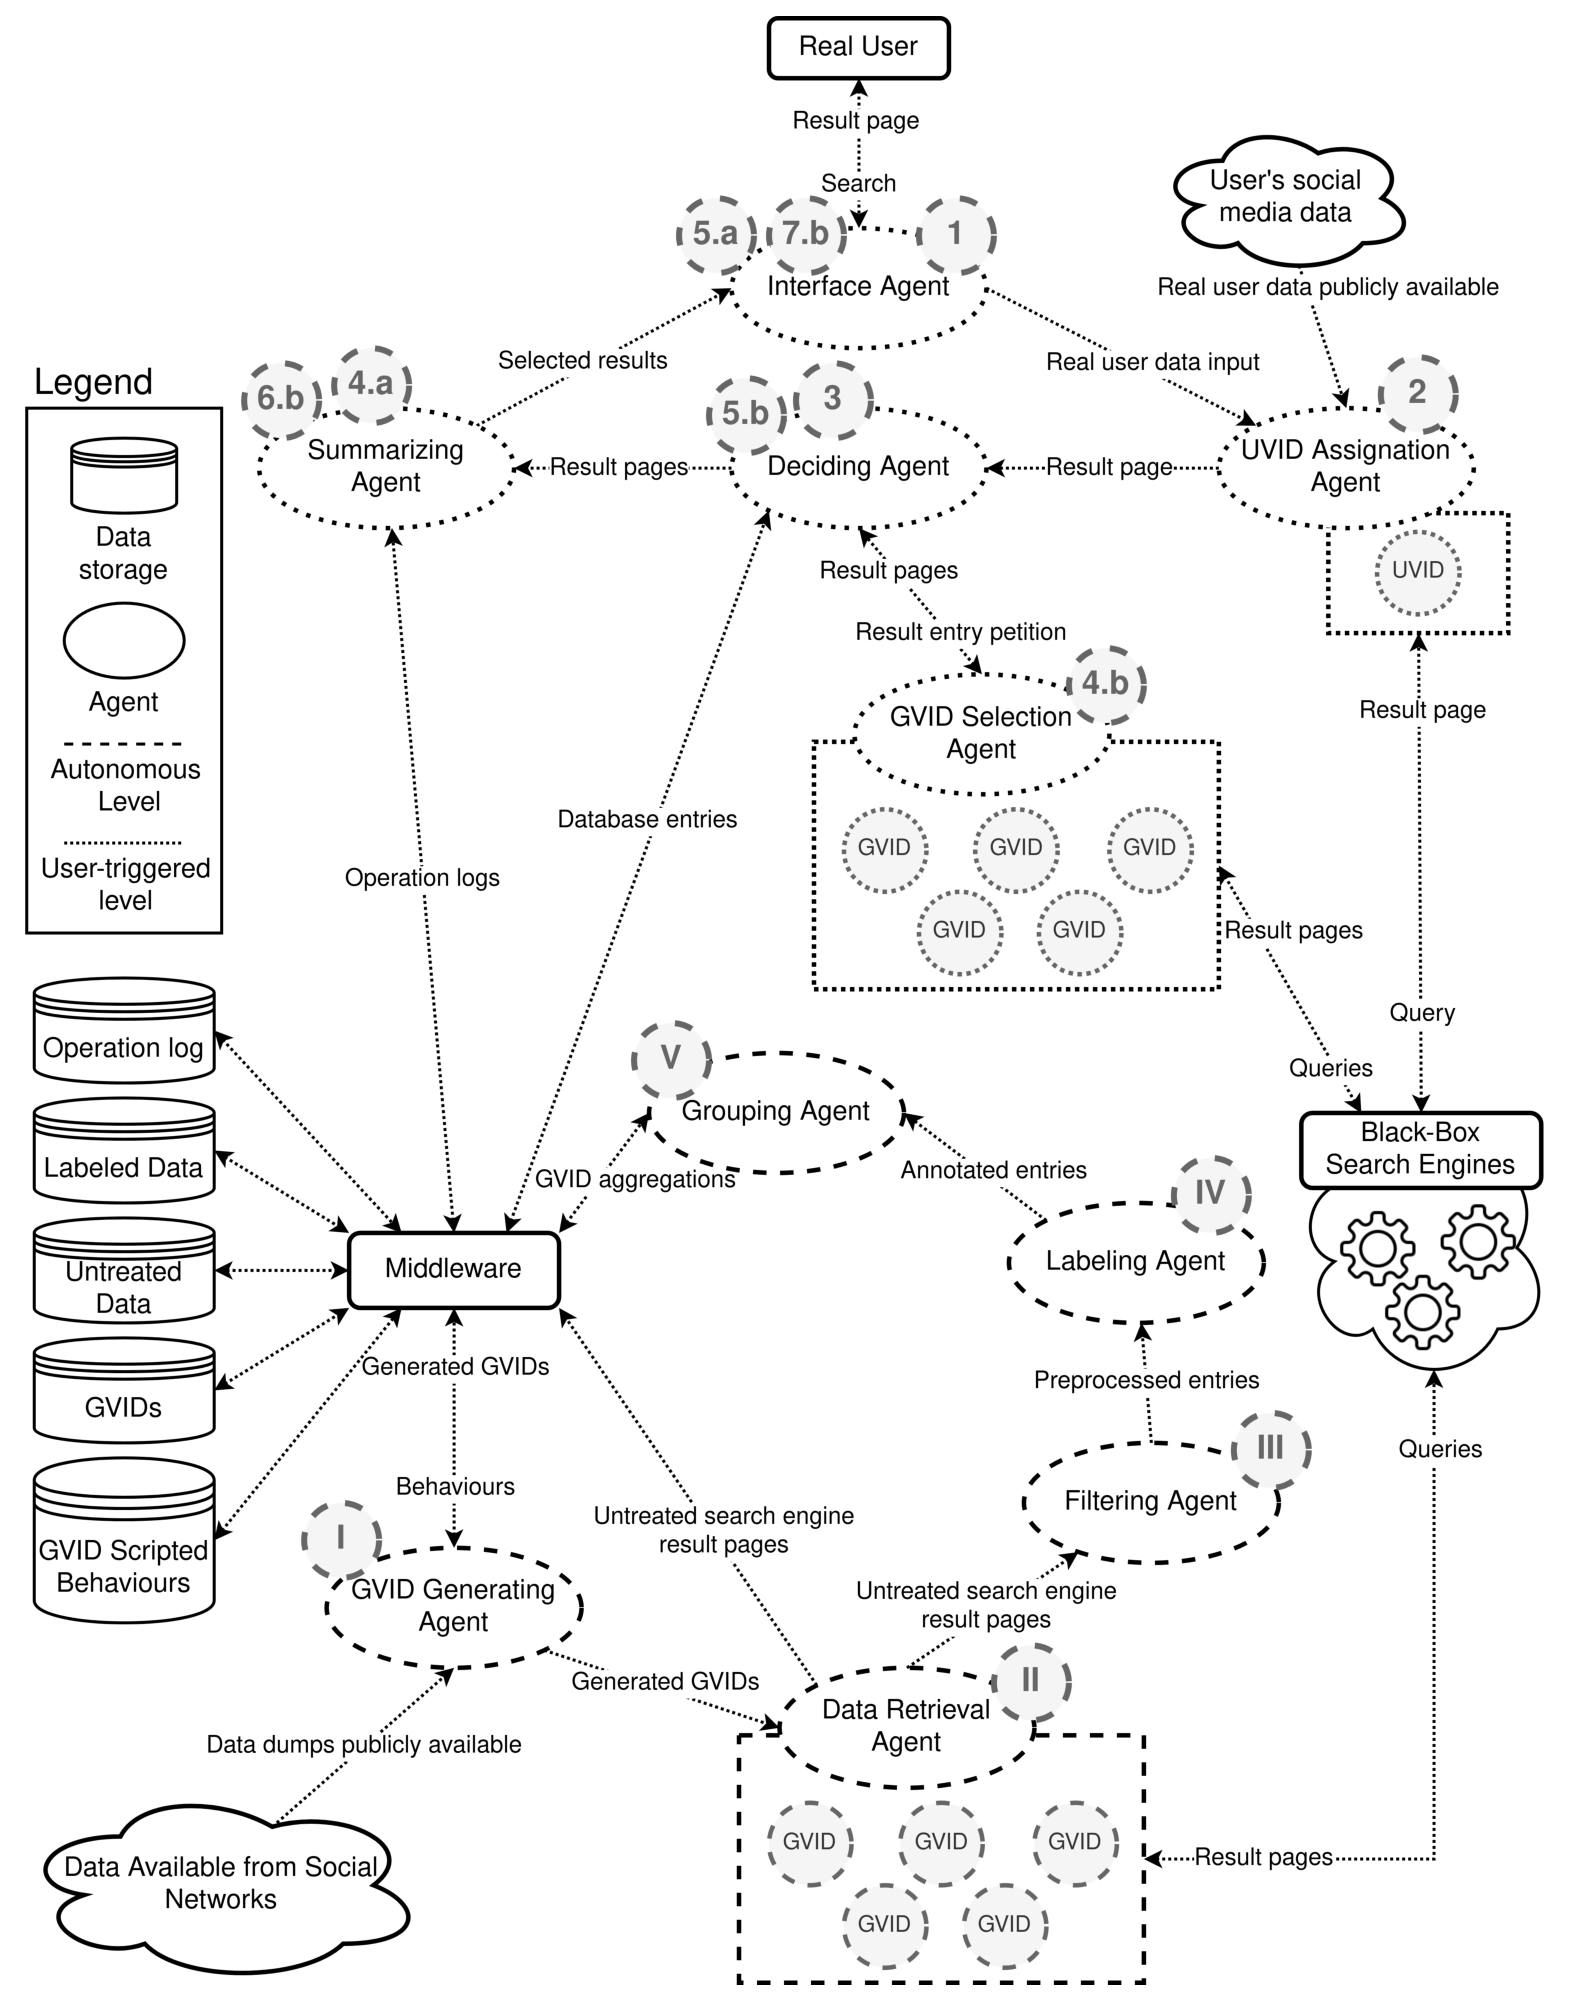
\includegraphics[width=.89\linewidth]{6_kbsextractiondl/figures/Use_Case.eps}
    \caption{Use case of the proposed architecture.}
    \label{fig:mas_use_case}
\end{figure}

The case study focuses on the analysis of the behavior of search engines. Specifically, on the relevance of the entries on the first result page. From the perspective of the user, the results that best fit the search query should be featured on the initial result page, independently from the employed search engine. However, this statement is not consistently met across search engines as the result may vary not only between search engines, but also between users. Moreover, most search engines feature advertising content amongst the top results, even when this content is unrelated to the search query. Therefore, this content should be detected and replaced by relevant result entries.

The considered case scenario meets the following specifications:
\begin{itemize}
    \item The goal of the system is to detect, analyze, and optimize result entries in search engines.
    \item Multiple search engines are selected, acting as the BBHOS.
    \item A reduced set of GVIDs is selected. Each GVID has distinct features to maximize heterogeneity in the BBHOS results.
    \item The system determines which results are related to the user's query, removing those entries that contain unrelated content, such as adverts.
\end{itemize}

As the architecture is divided into two distinct levels, the interactions between the agents on each level are presented separately. Figure \ref{fig:mas_use_case} illustrates the present use case. Operations related to the autonomous layer are numbered using Roman numerals, while Arabic numerals denote the operations user-triggered layer. Two distinct scenarios can occur based on the outcome of the \textit{deciding agent}, identified with letters \textit{a} and \textit{b} to designate the execution order of the agents.

\subsubsection*{Autonomous level}
In this level, the system gathers data from different search engines to be processed by the agents. The workflow is as follows:

\begin{enumerate}[label=\Roman*.]
    \item The \textit{GVID generating agent} collects the available social network user data dumps and extracts a set of \textit{N} GVID behaviors from the database. The collected social network data is then shuffled and distributed into \textit{N} different sets, each containing information such as tweets, reviews or opinions. Sentiment analysis and topic modeling are then performed over the sets to extract interest and opinions. This information is then combined with the GVID scripted behaviors to generate the final GVID set. The generated GVIDs are then stored in the database.
    
    \item Once the GVIDs are created, the \textit{data retrieval agent} selects a set of search engines to act as BBHOS, as well as defining the browsing terms to be queried. The browsing term set is composed by the topics extracted in the prior step. Each GVID does the same number of searches, and multiple GVIDs query the same term across the different engines. This enables the analysis of the results returned when the same term is browsed on different search engines and those obtained by different GVIDs when the search terms and engine are the same. The obtained responses are stored in the corresponding database.
    
    \item The result pages received by the GVIDs are then forwarded to the \textit{filtering agent}, which performs the data preprocessing. The collected data is in HTML format, thus containing several moot elements, such as markup text, references or symbols. The following operations are performed to clean the raw result pages: entry extraction, HTML and JavaScript markup removal, empty word removal and non-alphanumeric character removal. A set of clean result entries is obtained as outcome.
    
    \item As previously stated, search engines tend to merge advertising and valid result entries within the same page. Invalid entries should be detected and discarded, such that the user is only presented with entries that correspond to valid search results. The \textit{labeling agent} receives the result entry set from the previous agent and classifies entries into real result and advertisements. This problem can be subsequently treated as binary text classification. Labeled result entries are stored in the labeled data storage.
    
    \item Finally, GVIDs are hierarchically aggregated by their result entries to further analyzed the behavior of the search engines. The \textit{grouping agent} receives labeled entries and aggregates them following a hierarchical approach. As a result, GVIDs are grouped based on the result entries provided for each of them by the different engines. Information about the behavior of the search engines can then be extracted, such as which profiles are the most prone to receive advertising content, which engine includes the least amount of irrelevant content amongst its entries, or whether the results provided by the same engine on the same search vary across GVIDs. GVID aggregations are also saved in the GVID database.
\end{enumerate}

\subsubsection*{User-triggered level}
Once the autonomous level finishes its execution, the system remains suspended until a user makes a request. In this example, the request is a search query that the user inputs into a search engine. When the user makes the request, the user-triggered level of the system initiates its execution:
\begin{enumerate}
    \item The \textit{interface agent} collects the user's query, alongside with the needed user information. This input is sent to the \textit{UVID assignation agent} for further processing.
    
    \item The user's virtual identity, or UVID, is generated from the contextual information of the user, alongside with the publicly available social media information. The same procedure followed to generate the GVIDs is employed to generate the UVID. The UVID makes the user's search request, hindering the search engine from extracting contextual information about the user that could result in a privacy breach or lead to unfitting responses.
    
    \item The UVID executes the user's search query on the search engine. Then, the \textit{deciding agent} receives the result pages, determining whether the entries returned by the engine fit the user's request. Result entries are extracted from the result page to analyze their validity. These entries are filtered following the same procedure from step III. Then, the text classification model is used to discern advertisements from real result entries. At this point, two different scenarios can occur based on whether the result entries are real results (\textit{Scenario A}) or not (\textit{Scenario B}). 
    
    \paragraph{Scenario A}
    \begin{enumerate}
        \item [4.a] If the results provided by the engine to the UVID are relevant, meaning that no advertisements have been detected within the entries, the \textit{summarizing agent} compiles them for the user (e.g., removes duplicate entries).
        
        \item [5.a] Finally, the \textit{interface agent} builds a result page from the final result entry set and displays it to the real user. The constructed result page is formatted employing an adequate layout to present the information to the user in a clear and comprehensible way.
    \end{enumerate}
    
    \paragraph{Scenario B}
    \begin{enumerate}
        \item [4.b] If there is unrelated content amongst the results, the \textit{deciding agent} discards those entries and makes a petition to the \textit{GVID selection agent} to obtain new, valid entries to replace the removed ones. A set of GVIDs is selected following the hierarchical selection criteria, repeating the same query on the search engine. The new responses are sent back to the \textit{deciding agent}.
        
        \item[5.b] The new set of entries obtained by the GVIDs is analyzed by the \textit{deciding agent}, following the procedure presented in the step 3. The results that better fit the search query are then selected to replace the discarded entries. If no relevant results are found, the agent makes a new petition to the \textit{GVID selection agent}, repeating the process until valid result entries are obtained.
        
        \item [6.b] The generated result entry set, composed by the entries received by the UVID and the GVIDs, is transferred to the \textit{summarizing agent}. Aside from summarizing the result entries, this agent also generates a log comprising the operations required to obtain the final result entry set, identifying the GVID that originated each result.
        
        \item [7.b] The \textit{interface agent} composes a result page from the final entry set and displays it to the user, finishing the execution of the user-triggered layer of system.
    \end{enumerate}
\end{enumerate}

\subsection{Design Compliance}\label{6_sec:subsec:mas_design_compliance}
Section \ref{6_sec:mas_bbhos_general} introduces a hierarchical multi-agent system to extract behavioral patterns and improve user privacy in BBHOS, powered by DL. Figure \ref{fig:compliance_mas_extra_dl} depicts the specific design parameters of the presented use case:
\begin{figure}[t]
    \centering
    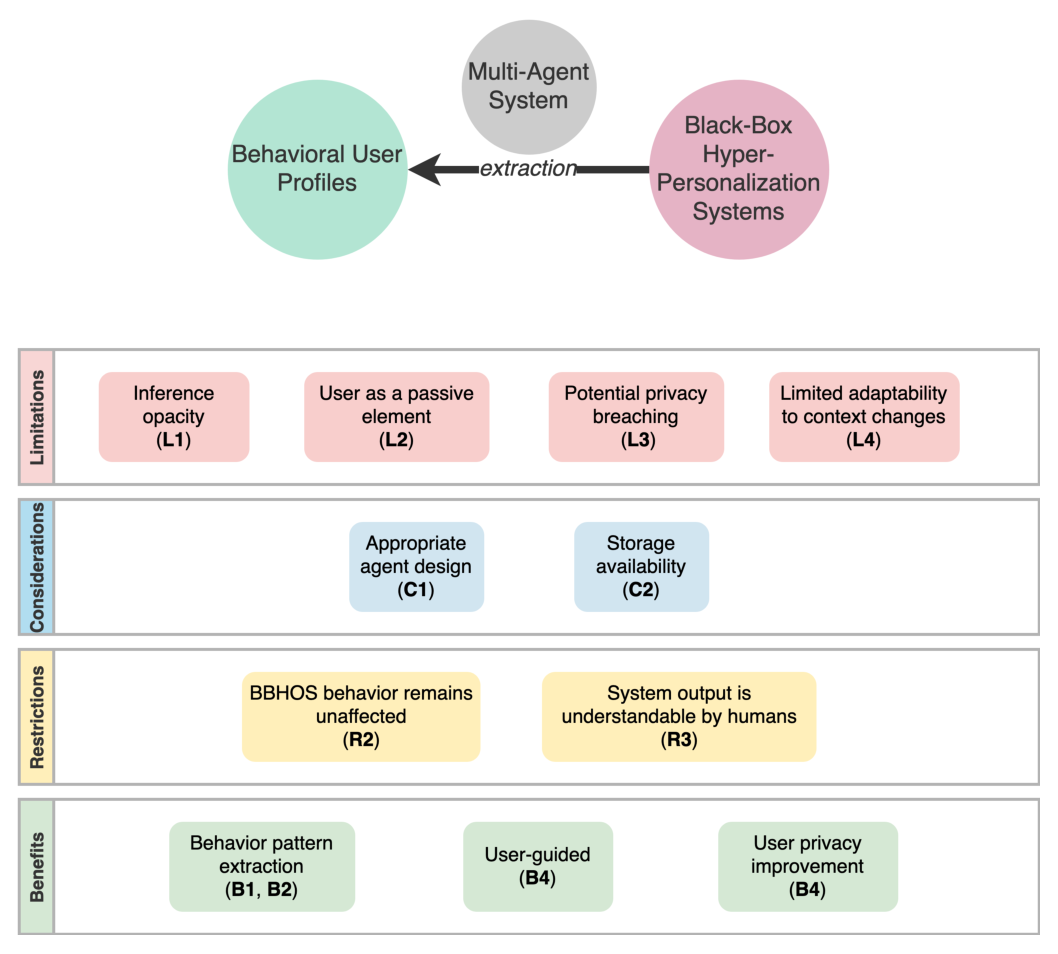
\includegraphics[width=\linewidth]{6_kbsextractiondl/figures/Instance_MAS_K_extraction_DL.eps}
    \caption{Overview of the design parameters of MAS extraction on BBHOS. In bold, the general design parameters as depicted in \ref{fig:kbs_extra_dl_overview}.}
    \label{fig:compliance_mas_extra_dl}
\end{figure}

\subsubsection*{Limitations}
\begin{itemize}
    \item \textbf{Inference opacity.} BBHOS are opaque by default. From a user perspective, the unawareness of why a content is targeted may prevent trust building. From a technical standpoint, opacity hinders the transferability of the model (\ref{kbsextradl_L_opacity}).
    
    \item \textbf{User as a passive element.} Even though the user is the core element of personalization, their role in BBHOS is entirely passive. The user is targeted on personalized content, but not actively inquired on its appropriateness. Instead, it is devised based on data that is collected unknowingly from the user (\ref{kbsextradl_L_human}).
    
    \item \textbf{Potential privacy breaching.} BBHOS rely on user-generated data to generate personalized, targeted content. While the user may initially give consent to provide their data, they may not be aware of its implications. Such is the case of microphone-collected data, where the user may not be conscious of being recorded, and subsequently can feel its privacy invaded when the BBHOS provides recommendations based on this data (\ref{kbsextradl_L_ethical}).
    
    \item \textbf{Limited adaptability to context changes.} BBHOS systems rely entirely on input data. This data is heterogeneous, reflecting diverse information. Some of this information may be actually relevant and reflect a change in the user context, while other may be misleading and induce noise into the BBHOS (\ref{kbsextradl_L_transferability}). 
\end{itemize}
\subsubsection*{Considerations}
\begin{itemize}
   \item \textbf{Appropriate agent design.} One of the main challenges in multi-agent systems is the agent design. In this scenario, the goal is to extract behavior patterns of BBHOS about their interactions with users and use them to improve the user's privacy and provide a better output. Agents must be devised to pursue this goal, thus ensuring that human-like behaviors are correctly emulated and accurate behavioral profiles can be extracted (\ref{kbsextradl_C_paradigm}).
    
    \item \textbf{Storage availability.} The proposed architecture comprises several storage units, each dedicated to a specific outcome. The storage capacity required may increase with subsequent system executions. Therefore, the availability of sufficient storage capacity must be guaranteed (\ref{kbsextradl_C_resource}).
\end{itemize}
\subsubsection*{Restrictions}
\begin{itemize}
    \item \textbf{BBHOS behavior remains unaffected.} One of the goals of the proposed MAS is to analyze the behavior of the BBHOS. Therefore, the BBHOS must remain unchanged to extract accurate insights and behavior patterns, as behavioral modifications can lead to inaccurate and erroneous conclusions (\ref{kbsextradl_R_behavior}).
    
    \item \textbf{System output is understandable by humans.} The user is at the core of the proposed MAS, being the main beneficiary. The output of the system must be aligned with this criterion, and therefore should be readable and understandable by humans (\ref{kbsextradl_R_human}).
\end{itemize}

\subsubsection*{Benefits}
\begin{itemize}
    \item \textbf{Behavior pattern extraction.} Opacity is one of the main setbacks of BBHOS. One of the main benefits of the proposed MAS is the capacity of extracting behavioral patterns from these opaque systems, identifying how the personalized content changes across different profiles and contexts. Behavioral patterns may not be enough to fully explain the inference process of BBHOS, but can provide some insight (\ref{kbsextradl_B_interpretability}). Moreover, these patterns can evidence existing biases amongst the types of content provided to different profiles (\ref{kbsextradl_B_bias}).
    
    \item \textbf{User-guided.} While users portray a passive role in BBHOS, in the proposed MAS the user is an active impactful element. The user initiates the execution of the top level of the system, and its interaction with the system conditions the behavior of the agents (\ref{kbsextradl_B_human}). 
    
    \item \textbf{User privacy improvement.} The behavioral patterns obtained by the MAS not only serve understandability purposes, but can be used to improve the user's privacy. The user is masked with an agent, which serves as a surrogate and interacts with the BBHOS. This agent can be modified accordingly to the user's goals and specifications to get better outcomes while simultaneously preventing the BBHOS to extract unwanted user data. 
\end{itemize}
%\section{A Hierarchical Multi-Agent Architecture Based on Virtual Identities}
\section{Generating Explainations and Insights on Knowledge Graph Embedding Predictions}\label{6_sec:geni_main}
%\section{Design Compliance I}
In Section \ref{4_sec:ontointro_kgc}, the introduction of ontologies into \textit{knowledge graph embedding} (KGE) models was explored to boost performance. Rules were also presented as an alternative to ontologies for semantic initialization, due to their capacity of encoding explicit and static restrictions about the data. However, in the existing rule integration approaches, the focus is on enhancing the model performance for \textit{knowledge graph completion} (KGC). Subsequently, the interpretability properties induced by the inclusion of rules within the model are not exploited. Therefore, KGE model explainability still remains a challenging issue. This Section presents a model-agnostic explainability framework for explaining knowledge graph embedding predictions.


\begin{sidewaystable}
\resizebox{\textwidth}{!}{
\begin{tabular}{|c|c|c|c|c|c|c|}
\hline
\textbf{Proposal} & \textbf{Type}   & \textbf{Baseline KGE Model} & \textbf{Constraints source} & \textbf{Goal of the proposal}                                                         & \textbf{Interpretable} & \textbf{Proposal focus} \\ \hline
\makecell{AMIE+ \\ \citep{amie+}}            & Rule-extraction & None                        & KG Data                     & Mine a set of rules from the KG                                                       & Yes                            & Output                  \\ \hline
\makecell{RUGE \\ \citep{ruge}}            & KGE Model       & ComplEx                     & KG Data + KG embeddings     & Enhance KGE performance                                                               & No                             & Input                   \\ \hline
RuleRec \citep{rulerec}          & Rule-extraction & None                        & KG Data                       & \makecell{Improve the performance of \\ recommendation systems while providing \\ explainable results} & Yes                            & Output                  \\ \hline
SLRE \citep{slre}             & KGE Model       & ComplEx                     & KG Data                     & Enhance KGE performance                                                               & No                             & Input                   \\ \hline
SoLE \citep{sole}             & KGE Model       & ComplEx                     & KG Data                     & Enhance KGE performance                                                               & No                             & Input                   \\ \hline
\makecell{pTransE\\ \citep{ptranse}}          & KGE Model       & TransE                      & KG Data                     & Enhance KGE performance                                                               & No                             & Input                   \\ \hline
TARE \citep{tare}              & KGE Model       & ComplEx                     & KG Data + KG embeddings     & Enhance KGE performance                                                               & No                             & Input                   \\ \hline
IterE \citep{tare}            & KGE Model       & ANALOGY                     & KG Data + KG embeddings     & Enhance KGE performance                                                               & No                             & Input \& Output                  \\ \hline
RuLES \citep{ruLES}           & Rule-extraction & None                        & KG Data + KG embeddings     & Mine a set of rules from the KG                                                       & Yes                            & Input \& Output         \\ \hline
KALE \citep{kale}             & KGE Model       & Translation-based           & KG Data + external sources  & Enhance KGE performance                                                               & No                             & Input                   \\ \hline
RBox \citep{rbox}             & KGE Model       & Translation-based           & External sources            & Enhance KGE performance                                                               & No                             & Input                   \\ \hline
\cite{yoonetal}      & KGE Model       & Translation-based           & Non-declared                & Enhance KGE performance                                                               & No                             & Input                   \\ \hline
RLvLR  \citep{rlvlr}           & Rule-extraction & None                        & KG Data + KG embeddings     & Mine a set of rules from the KG                                                       & Yes                            & Input \& Output         \\ \hline
\makecell{HyperKG\\ \citep{hyperkg}}          & KGE Model       & Translation-based           & KG Data                     & Enhance KGE performance                                                               & No                             & Input                   \\ \hline
RPJE \citep{rpje}              & KGE Model       & Translation-based           & KG Data                     & \makecell{Enhance KGE performance and \\ improve its interpretability}                              & Yes                            & Input \& Output         \\ \hline
\makecell{AnyBURL\\ \citep{anyburl}}          & Rule-extraction & None                        & KG Data                     & Extract a set of rules from KG                                                        & Yes                            & Input \& Output         \\ \hline
UKGE \citep{ukge}             & KGE Model       & DistMult                    & Uncertain KG Data           & Enhance KGE performance                                                               & No                             & Input                   \\ \hline
\makecell{r-TransE\\ \citep{rtranse}}         & Hybrid Model    & TransE                      & KG Data + Embeddings        & \makecell{Integrate embeddings and rules\\ into a unified framework for \\ KG Completion}             & Yes                            & Input \& Output                  \\ \hline
\makecell{CrossE\\ \citep{crosse}}        & KGE Model       & Translational Models        & KG Data                     & Development of an explainable KGE Model                                               & Yes                            & Input \& Output         \\ \hline
\makecell{DRUM\\ \citep{drum}}          & Rule-extraction & None                        & KG Data                     & Extract a set of rules from KG                                                        & Yes                            & Input \& Output  \\ \hline  
\end{tabular}  
 \caption{An overview of the existing approaches that combine rule- and embedding-learning methods.}
\label{tab:rules_kg}
}
\end{sidewaystable}

Table \ref{tab:rules_kg} provides an overview of the existing hybrid models that integrate rule-based systems and KGE. CrossE \citep{crosse} is also included despite not using rules, as it is one of the few existing KGE models that explicitly considers explainability. Two tendencies can be detected among the models presented in Table \ref{tab:rules_kg}: rule mining and KGE performance boosting. The first tendency applies only to rule-learning models, where rule-learning takes the primary role. In these models, KGE supports the confidence validation and assessment of the extracted rules, as well as assisting in pruning and ranking. As rule-learning models aim to mine rules from the KG, their focus is not on the input data, but on the validation of the model's results.

\begin{figure}[t]
    \centering
    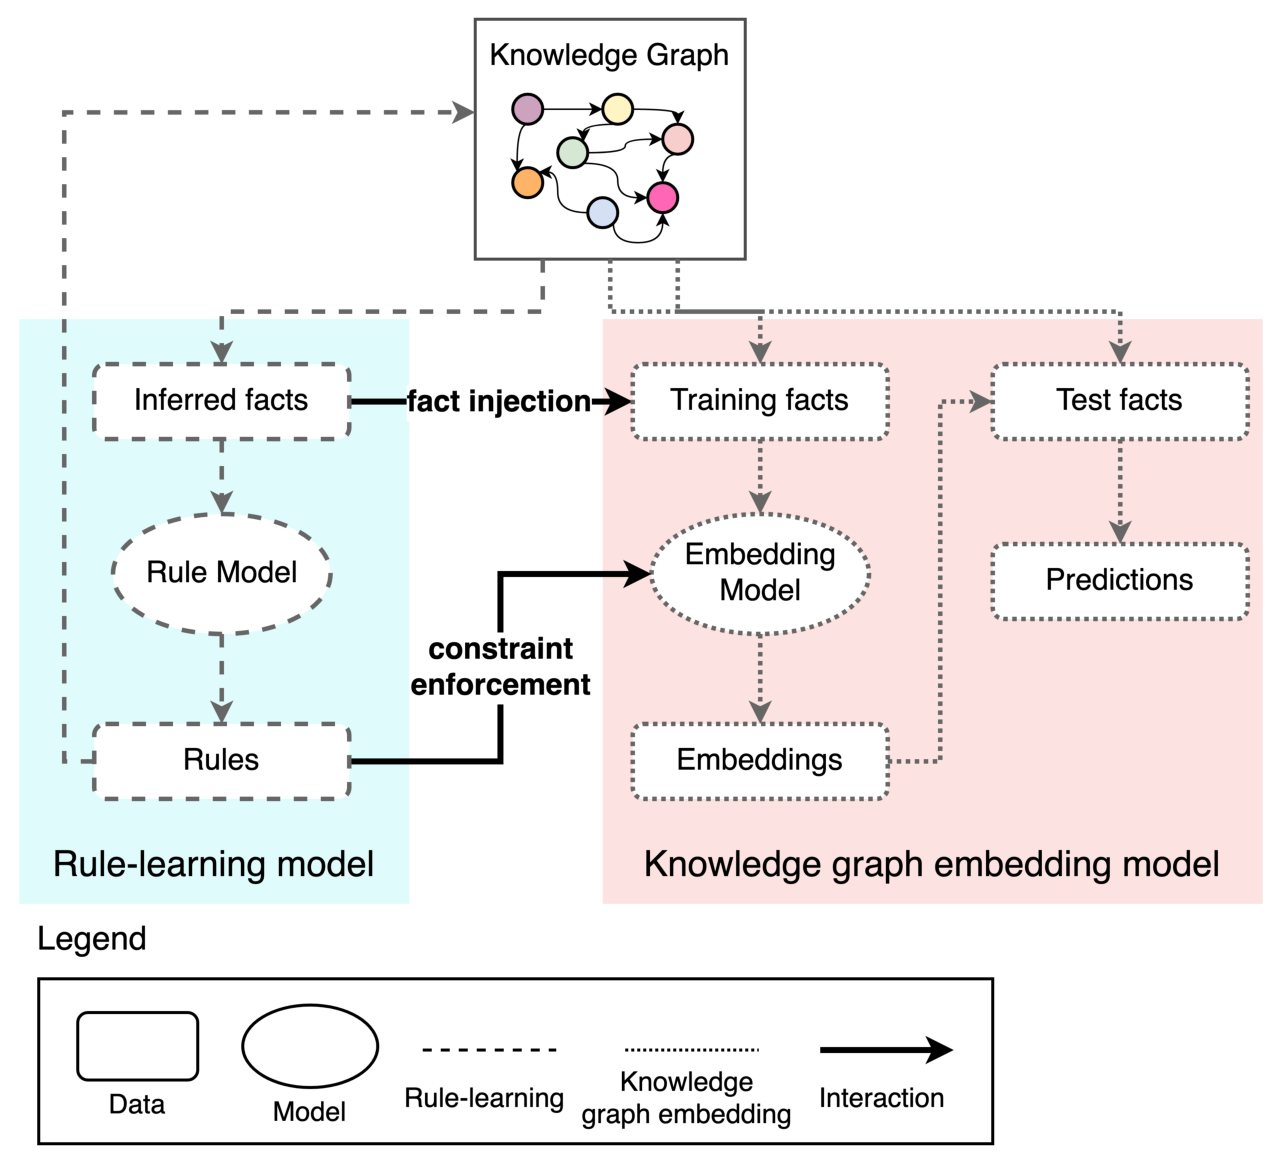
\includegraphics[width=.7\linewidth]{6_kbsextractiondl/figures/rule_support_training.eps}
    \caption{General workflow of a knowledge graph embedding model training with rule-based support.}
    \label{fig:rule_training}
\end{figure}

Several embedding-learning models incorporate rules as a supporting element to improve performance. In this scenario, the benefits of rule introduction are twofold: increasing the number of available training facts through rule instantiation and enforcing explicit constraints between relations. Furthermore, while rule-learning methods iteratively refine the results provided by the model, embedding-learning strategies focus on improving the input so that the improvements are propagated throughout the model and reflected in the final results. Figure \ref{fig:rule_training} depicts the general workflow of a rule-supported KGE model. As depicted, rules are only considered during model training. Therefore, the focus is on boosting the performance of the model instead of explaining the final predictions.

Data augmentation approaches rely on rule mining models, such as AMIE+ \citep{amie+}, to extract a set of rules from the KG. The generated rules can then be instantiated with the KGE training facts, leading to new facts. Increased data availability during training leads to improved final results. In those cases where the focus is on learning and imposing relation constraints, rules and restrictions are computed alongside the embeddings. Rules are then used to evaluate the consistency of the embeddings. The final embeddings encode rule restrictions, leading to better predictions.

As reported in Table \ref{tab:rules_kg}, only two of the studied KGE models are capable of providing interpretable results. This is directly related to the training paradigm of KGE models, where the goal is to improve the accuracy and performance of the model across different metrics. Moreover, most of the reported KGE enhancement proposals are only suitable for specific models, hindering its reusability.

\cite{bianchi_kge_explainability_2020} presents a study on the explainability of KGE models. As denoted in this work, defining explainability in this context is not trivial, as there is not an agreed definition. In the context of KGE, any potential information that can accurately relate the model prediction to both the input data and the embeddings can be regarded as an explanation. According to this definition, DistMult \citep{distmult} was one of the first attempts of introducing explainability in KGE models. In addition to providing a novel KGE proposal, DistMult also presents a method for the generation of Horn clauses from embeddings. Moreover, this work introduced a novel perspective on rule mining: replacing the KG with the embeddings as the data source. This change of paradigm not only solves one of the main issues in rule-mining models (search space optimization), but also provides a novel and data-agnostic vision on the subject.

\subsection{GEnI: A Knowledge Graph Embedding Model-Agnostic Framework}\label{6_sec:subsec:geni}
This Section introduces GEnI: a three-level, model-agnostic explainability framework. Following the guidelines established in DistMult, the first mainstay of the approach is that \textit{all insights on the inference process of the model should be extracted from the embeddings, not the data}. This criterion ensures that the proposal strictly explains the model output, and not the KG itself. This approach also relates the quality of feasible explanations to the performance of the KGE model. Therefore, if the model produces accurate predictions, GEnI may also provide an insight on the inference that leads to the output. On the contrary, if the KGE model has a subpar performance, no information on the output may be inferred. Aligned with this principle, the second mainstay of the proposal is that \textit{the KGE model output is considered as a ground truth to be explained, independently on its rightfulness.}

\begin{figure}[t]
    \centering
    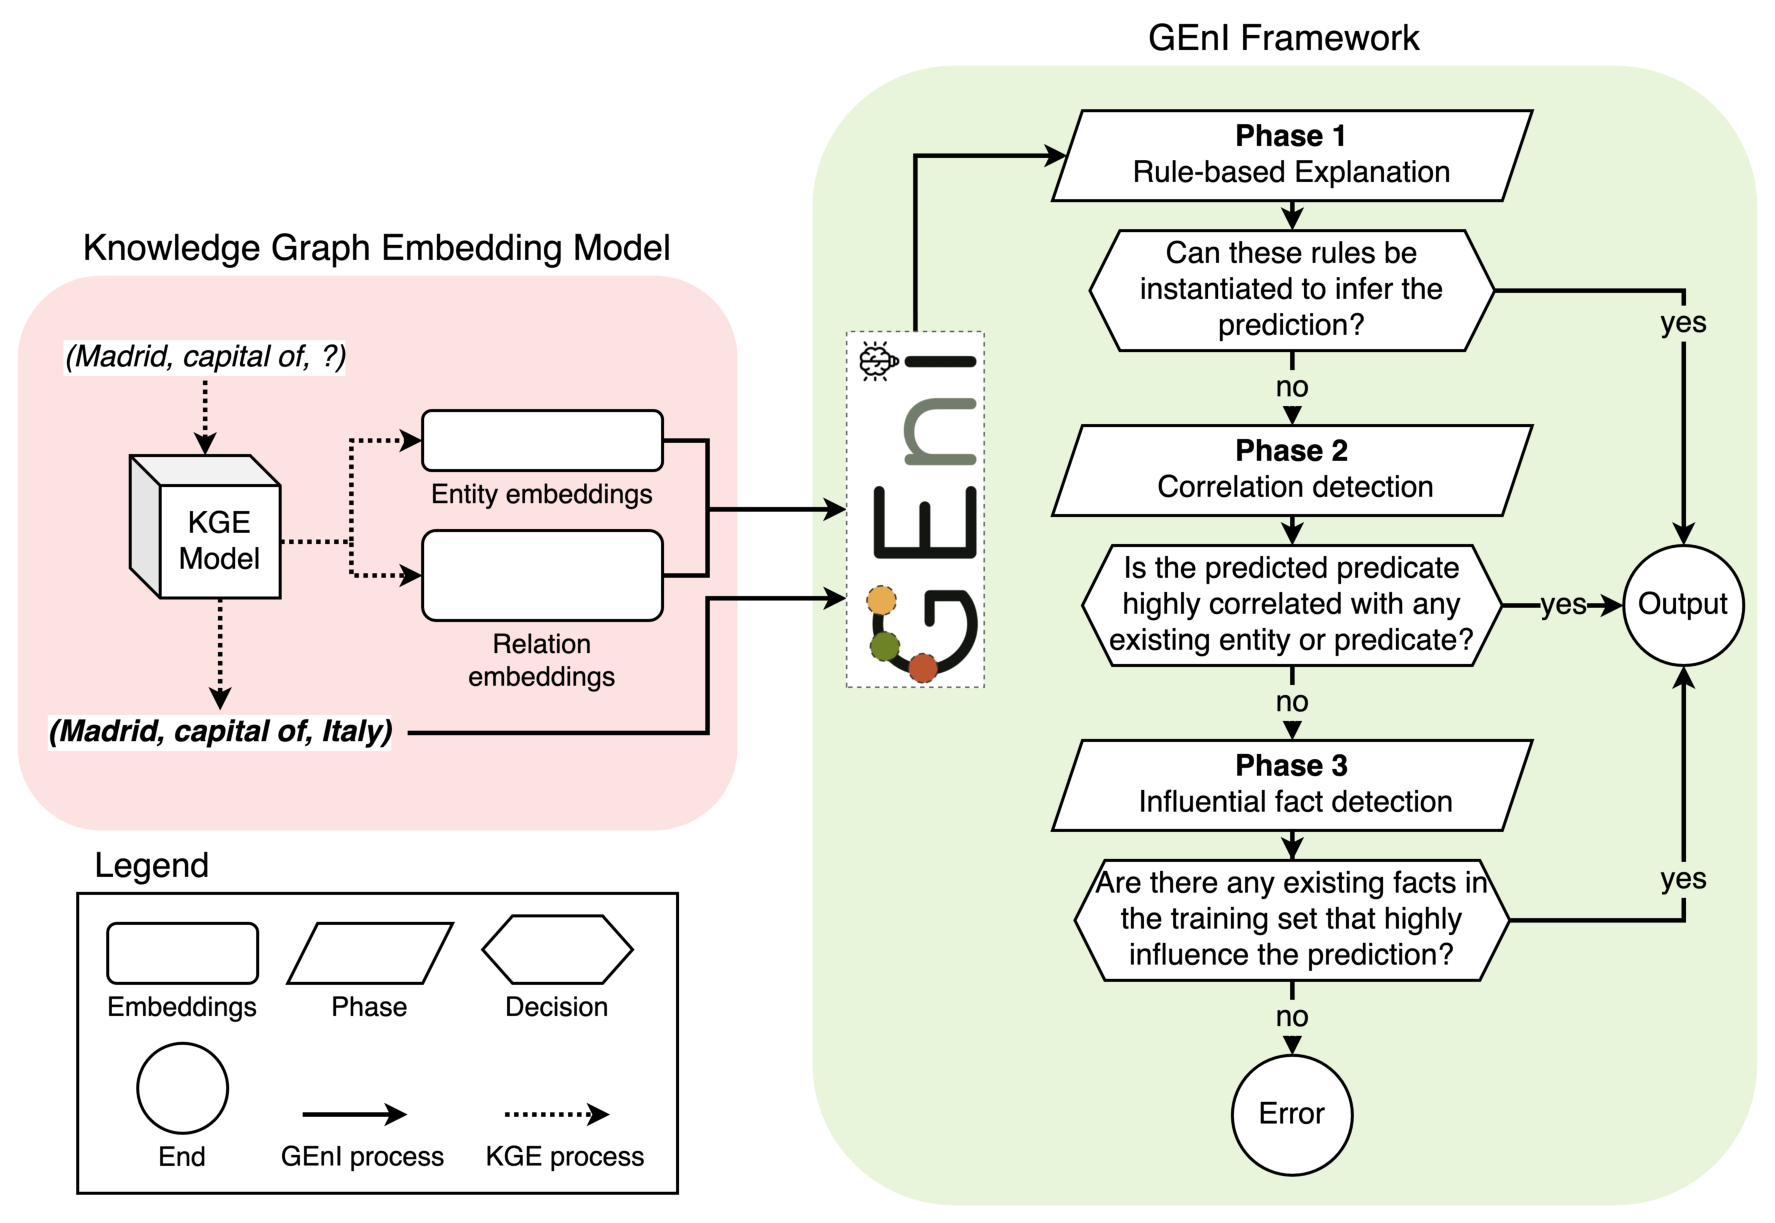
\includegraphics[width=\linewidth]{6_kbsextractiondl/figures/geni_overview.eps}
    \caption{Overview of the proposed KGE explainability framework}
    \label{fig:overview_geni}
\end{figure}

Figure \ref{fig:overview_geni} showcases the general behavior of the framework. First, the KGE model generates a prediction on a given input fact. In the example, the KGE model is inquired about the fact \textit{(Madrid, capital of, ?)}, to which the provided response is \textit{Italy}. The framework then aims to provide an insight on why the fact \textit{(Madrid, capital of, Italy)} is inferred. The explaination process comprises three sequential phases, ranging from more general to more specific. 

In the first two phases, potential insights are extracted from a set of operations performed directly over the embeddings, which are then validated against the KG data. A criterion is established to decide which of the potential insights should be validated and presented to the user in case of success. From a general standpoint, insights are extracted by establishing a comparison between a given operation $O_p$ over the input fact and the results obtained from executing $O_p$ over the set of potential entities $\mathcal{E}'$ and relations $\mathcal{R}'$. Equation \ref{eq:general_restriction} draws the general restriction for insight extraction, where $|$ denotes the logical operator OR:

\begin{equation}\label{eq:general_restriction}
    Op(s,r,o)\approx [Op(\mathcal{E}') | Op(\mathcal{R}')]\,.
\end{equation}

Measuring the similarity between the results of the operations on both sides of the inequality is essential for extracting good insights. The elements of the equation can be either vectors or matrices depending on the phase and the KGE model. Therefore, different metrics are required to compute the similarity between both sides of the equation. Regarding vector operations, cosine similarity is the preferred choice, as it provides values in the range $[-1,1]$. For matrices, Frobenius norm is the standard comparison metric. However, since both metrics use different scales, as the Frobenius norm is a distance-based metric, Euclidean norm is used for vector comparison. 

Distance-based metrics are not bounded to a fixed range, which hampers the comparison between results. Moreover, the range of entity and relation embeddings depends on the KGE model, as well as on the initialization. A tolerance threshold is therefore specified to denote which is the maximum acceptable distance between two comparable components (matrices or vectors) to consider them similar. If the threshold value is too restrictive, no insights on the prediction may be found. Alternatively, low threshold values can lead to inaccurate insights while significantly increasing the computational time. The optimal threshold value can be empirically computed, but it must not be treated as a quantitative element, but a qualitative one. Therefore, the threshold value is specified by the user, introduced as a similarity value in the range $[0,1]$. This value is then rescaled and translated into the threshold $th\_value$ as follows:

\begin{align} 
   tolerance = max(\mathcal{G}_{embeddings})- min(\mathcal{G}_{embeddings}), \nonumber  \\
    th\_value = tolerance + ( 1 - sim\_ratio ) \times  tolerance,
\label{eq:threshold_value}
\end{align}

where $\mathcal{G}_{embeddings}$ is the values of all the embeddings (both entities and relations), and $sim\_ratio$ is the user-specified similarity ratio. Equation \ref{eq:threshold_value} ensures that the threshold value $th\_value$ is compliant with the embedding range and the similarity value specified by the user. Insight candidates are then filtered according to Equation \ref{eq:candidate_filter}:

\begin{equation}\label{eq:candidate_filter}
    dist( Op(s,r,o),  [Op(\mathcal{E}') | Op(\mathcal{R}')] ),
\end{equation}

where $O_p$ is the phase-specific operation and $dist$ the corresponding distance function (Euclidean or Frobenius). 

Similarly to rule-based models, efficiently traversing the search space to find the relevant elements is one of the key challenges. In rule-learning systems, search space optimization is performed using pruning and walking algorithms. However, these methods can not be applied in this scenario, where the search space is composed by a set of labeled embeddings. In rule-based models, axioms are mined from the detection of facts that share common elements, or whose relations feature similar entities. Although this criterion can not be directly applied to the proposed framework, an equivalent approach can be followed to compute related elements from the embeddings. Once trained, both entity and relation embeddings encode semantic information about their interactions with the graph components. KGE model training also ensures that entities and relations that have similar interactions lead to close embeddings in the resulting vector space. 
In the context of embeddings, search spaces can be envisioned as clusters generated under the aforementioned constraints. Therefore, elements with similar embeddings are grouped into the same cluster. Under this criterion, the search space for a given insight is composed of clusters of subject and object entities, as well as their predicates. Efficiently detecting these aggregations poses a considerable challenge, as the performance of most clustering approaches does not scale up with the dimension of the data. Both entity and relation embeddings have dimensions that exceed the hundred entries, which squares up for relation matrices. For high-dimensional data, operations such as principal component analysis may be required.

\subsubsection*{Phase 1: Axiom extraction from relation embeddings}

One of the core principles of the proposal, as previously stated, is that all explanations must stem from the embeddings, and not the data. Subsequently, embedding-based mechanisms capable of accurately extracting rules from the representations are required. IterE \citep{itere} presents the equivalence between OWL2 ontology axioms and their corresponding rule formulations. Seven axiom types are reported in the original work, but only five are considered in this proposal. The reflexive property is not considered, as KGs should not include self-loops, thus making this property unfeasible.  The sub-object property is also removed due to its redundancy with the equivalence property, as they both derive from the same rule form. Table \ref{tab:owl_restrictions} draws the relation between axioms, rule forms, and embedding restrictions in both translational and bilinear models. These models follow the scoring functions outlined in Section \ref{subsec:s4_theoretical_back}. While each KGE model introduces variations with respect to the baseline function, the generated embeddings are still compliant with the baseline scoring functions. These functions can then be used to infer general restrictions about the embeddings that are equivalent to the studied axioms, as outlined in Table \ref{tab:owl_restrictions}. These restrictions can be used to identify rules directly from the embeddings.

\begin{table}[t]
\resizebox{\linewidth}{!}{
\begin{tabular}{cccc}
\textbf{OP Axioms}      & \textbf{Rule Form}              & \makecell{\textbf{Bilinear}\\\textbf{Restrictions}} & \makecell{\textbf{Translational}\\\textbf{Restrictions}} \\
SymmetricOP($r$)          & $(y,r,x)\leftarrow(x,r,y)$                 & $M_r M_r \simeq I$                          & $v_r+v_r \simeq 0$                           \\
TransitiveOP($r$)         & $(x,r,z)\leftarrow(x,r,y),(y,r,z)$         & $M_r M_r \simeq M_r$                         & $v_r+v_r \simeq v_r$                           \\
EquivalentOP($r$)         & $(x,r_2,y)\leftarrow(x,r_1,y)$               & $M_{r_1} \simeq M_{r_2}$                         & $v_{r_1} \simeq v_{r_2}$                           \\
InverseOP($r_1,r_2$)        & $(x,r_1,y)\leftarrow(y,r_2,x)$               & $M_{r_1} M_{r_2} \simeq I$                        & $v_{r_2}+v_{r_1} \simeq 0$                         \\
ChainOP(ChainOP($r_1,r_2$),$r$) & $(x,r,z)\leftarrow(x,r_1,y),(y,r_2,z)$ & $M_{r_1} M_{r_2} \simeq M_r $                       & $v_{r_1}+v_{r_2} \simeq v_r$                        
\end{tabular}}
\caption{Relation of object properties with their corresponding rule forms. Inferred mathematical restrictions under the two KGE assumptions (Bilinear and Translational) are provided. $M$ and $v$ denote the relation matrices and vectors, respectively.}
\label{tab:owl_restrictions}
\end{table}

When a new fact $(s,p,o)$ enters the framework, the embedding of the predicate $p$ is retrieved. First, symmetry and transitivity are evaluated according to their restriction operations. The threshold value $th\_value$ is used to establish whether the inequality holds. If the restriction is met, the corresponding axiom is considered for further evaluation. The same process is followed for the remaining properties. Efficiently and accurately detecting which relations in $\mathcal{R}$ are the closest to $p$ is the main challenge of this phase. Usually, the number of relations in a KG is pretty limited. K-means can be used to detect neighbouring relations, where the optimal value of $k$ is computed via gap-statistic optimization. While k-means provides a simple and effective solution, it does not accurately capture the KG, as it only assigns a single cluster per relation. C-means poses a fuzzy alternative to k-means, based on the same aggregation criteria but considering the possibility that an element can belong to more than one cluster. Additionally, it can automatically estimate the optimal number of clusters. C-means is selected as the neighbour detection method for relations.

Once predicate $p$ is evaluated on all properties, a set of potential rules is obtained. At this stage, the rules are not instantiated, and subsequently it can not be ascertained whether the input fact can be inferred from them. Potential rules are then evaluated on the KG facts. In this evaluation, potential rules are instantiated to find a feasible inference for the input fact. If a valid instantiation, it is returned to the user and the execution finishes. Second phase is initiated if no rules or instantiations are found.

\subsubsection*{Phase 2: Correlation between predicates}
In the first phase, only the predicate is considered. The second phase also includes entity information, being an intermediate solution between the general information provided by rules and the specificity of influencial fact detection. 

For some facts, the information on the predicate $p$ may not be sufficient to generate an insight on the inference process, as none of the properties in Table \ref{tab:owl_restrictions} may be observed. However, when combined with either the subject or object entity representation, $e$, a degreee of similarity can be observed between the obtained representation and those obtained by performing the same operation on the relation set $\mathcal{R}$ and the subset of entities related to $e$ denoted as $\mathcal{E}'$.

In the previous phase, c-means was sufficient to detect neighbouring relations efficiently and accurately, due to the limited number of elements. For entities, c-means can be ineffective due to the elevated number of elements, which can lead to a high number of single-element clusters which do not comprise a valid search space. Agglomerating hierarchical clustering is used as an alternative in this phase. First, the pairwise distance matrix is computed, measuring the Euclidean distance between each possible pair of entities in $\mathcal{E}$. From this matrix, entities are then aggregated using an agglomerating criterion that prioritizes the maximization of elements within each cluster. The set of closely related entities $\mathcal{E}'$ for an entity $e$ is the entities contained in its own aggregation.

\begin{figure}[t!]
    \centering
    \subfigure[Direct Correlation \label{fig:direct_corr}]{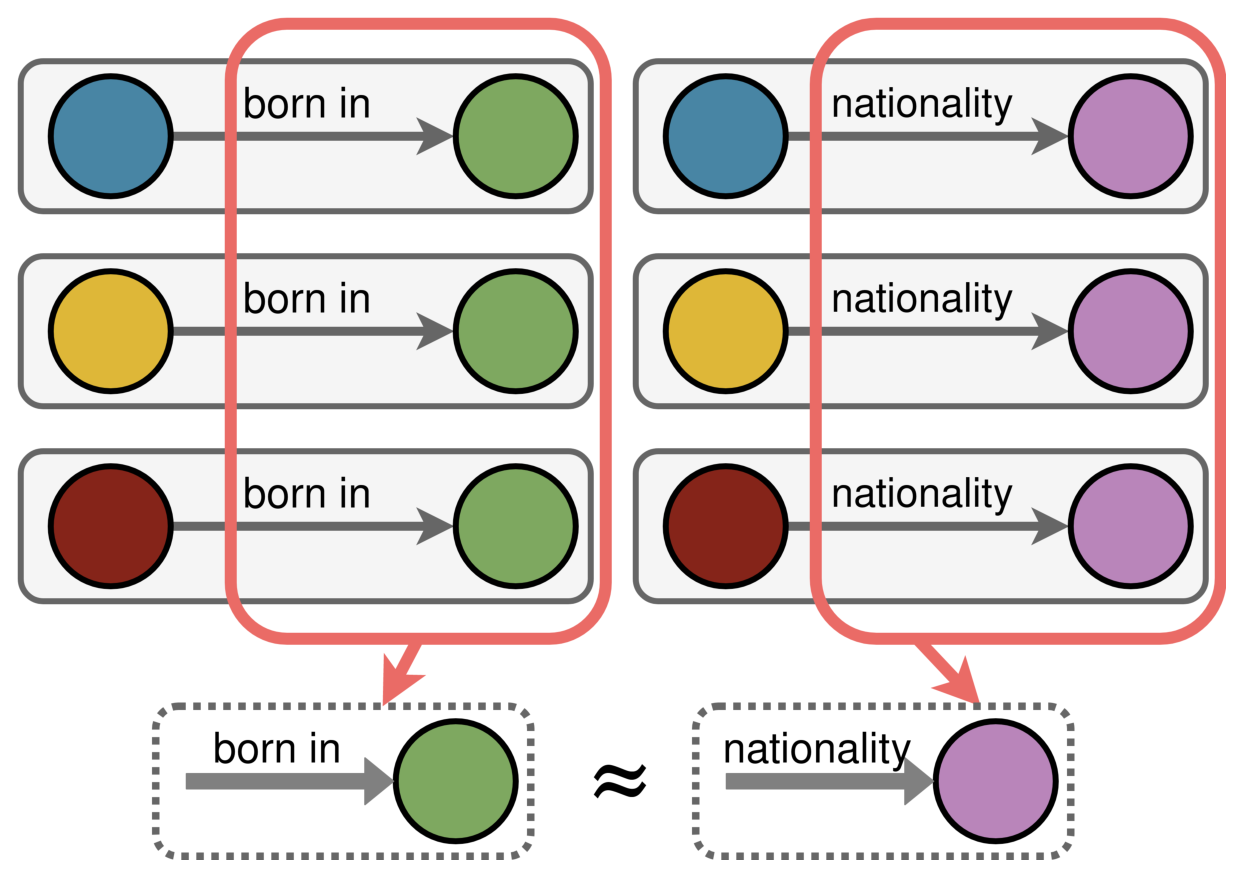
\includegraphics[height=1.7in]{6_kbsextractiondl/figures/direct_corr.eps}}
    \qquad
    \subfigure[Triangular Correlation \label{fig:triangular_corr}]{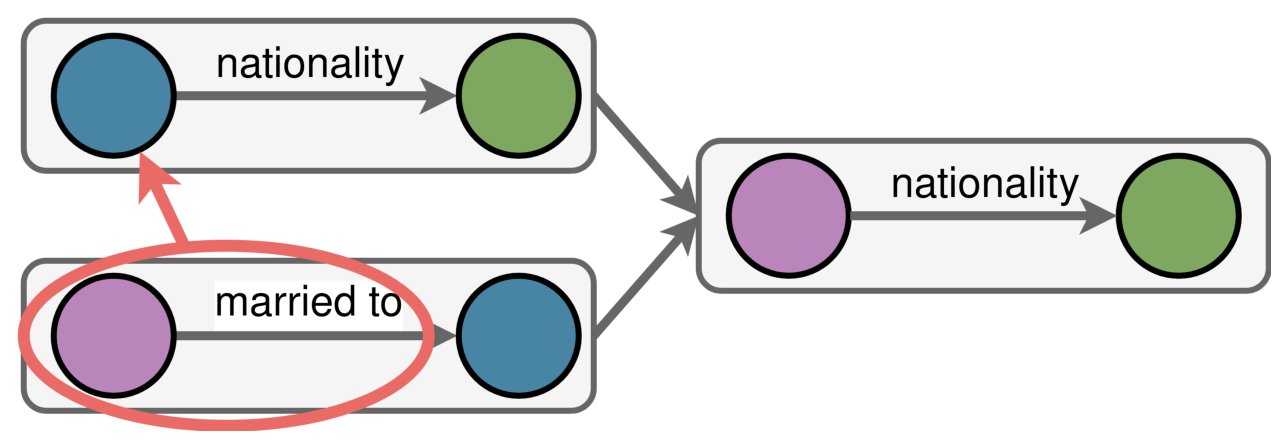
\includegraphics[height=0.9in]{6_kbsextractiondl/figures/triangular_corr.eps}}
    \caption{Overview on the two types of predicate correlations.}
    \label{fig:corr_overview}
\end{figure}

Figure \ref{fig:corr_overview} depicts the two types of correlations that can be identified based on the interactions between $\mathcal{E}'$ and $\mathcal{R}$ for the input fact.

\paragraph{Direct correlation}
In some cases, the inference of a particular entity $e$ can be explained based on the existence of a \textit{(relation,entity)} tuple that frequently features not only $e$, but closely related entities in $\mathcal{E}'$. As depicted in Figure \ref{fig:direct_corr}, \textit{direct correlations} are a widespread occurrence in relation pairs such as \textit{born in} and \textit{nationality}, as people from a given country will most likely have the same nationality. In these scenarios, where a pair of predicates $(X,r_1,e_1)$ and $(X,r_2,e_2)$ frequently feature the same entities, the KGE model is likely to learn this correlation for future inferences.

The following operations are performed on an input fact $(s,p,o)$ to extract potential direct correlations. First, the embeddings of the relation $p$ and predicted entity $e$ ($s$ in subject prediction and $o$ in object prediction) are extracted. Then, the set of entities related to $e$, $\mathcal{E}'$, is retrieved. Each entity $e \in \mathcal{E}'$ is operated with each relation in $\mathcal{R}$ via addition (translational models) or multiplication (bilinear models). The result of this operation is a matrix $M$ with dimensions $E \times d$, where $E$ is the number of entities and $d$ is the embedding dimension. Entries in $M$ whose Euclidean distance to $p$ is equal or less than the threshold value $th\_value$ are considered as potentially direct correlations. 

The set of potential direct correlations is then evaluated on the KG, assessing whether the input fact can be inferred. In addition to providing insight on the inference of a given fact, detecting these correlations can also help identify data biases. Detecting and correcting these biases can improve the overall performance of the model.

\paragraph{Triangular correlation}

In \textit{triangular correlations}, the correlation is not established between pairs of tuples, but between a tuple and a single entity. Figure \ref{fig:triangular_corr} depicts an example of this correlation. This phenomenon is relatively common in cases with a lack of facts about the predicted entity $e$ during training. This correlation establishes that, when the number of facts containing the entity $e$ is limited, its representation can be replaced by the resulting embedding of operating its most related entity $e'$ with the relation $r'$ that links them.

Similar to direct correlation, the first step is to extract the set $\mathcal{E}'$ containing the entities closely related to $e$. Then, each entity $e' \in \mathcal{E}'$ is operated with the representation of the predicate $p$, generating a matrix $M$ of dimension $E \times d$. Those entries in $M$ whose Euclidean distance to $e$ is equal or less than the threshold value $th\_value$ are considered for evaluation.

In addition to the explainability provided by these correlations, their detection can also be used as an indicator of which entities are lacking information. Moreover, it can also boost KGE model training, as it indicates which triples may not be relevant and can therefore be removed from training. 

Detected correlations (triangular or direct) about the input fact are evaluated on the KG. If the evaluation succeeds, the system finishes its execution. 

\subsubsection*{Phase 3: Influential fact detection}
Phase 3 initiates, as illustrated in Figure \ref{fig:overview_geni}, when none of the previous two phases succeed. Instead of providing broad and general explanations that can be feasible for more than one fact, phase 3 generates insights that can only explain the given input fact. 

Influence functions measure the shift value of an estimator at a given point when a certain indicator changes. In the context of KGE, influence functions assess the impact that a fact has on a prediction. CRIAGE \citep{criage} presents an adaptation of the general influence function for its application to bilinear KGE models. CRIAGE uses the Taylor expansion to estimate the change in the score of a given fact by approximating the difference in the embeddings when a fact is added or removed. Equation \ref{eq:influence} defines CRIAGE variation on the baseline influence function, where $S(s,p,o)$ is the score of the fact $(s,p,o)$, $f$ denotes the model scoring function, $H_o$ is the Hessian matrix containing the second-order derivative of the loss with respect to the embedding of the object entity, and $\varphi$ is the sigmoid of the score.

\begin{equation}\label{eq:influence}
   \widetilde{S}(s,r,o)-S(s,r,o) = f_{s,r}[(1-\varphi){(H_o+\varphi(1-\varphi)f_{s',r'}^{T}f_{s',r'})}^{-1}f_{s',r'}^{T}].
\end{equation}

The goal of CRIAGE is to evaluate the robustness of a KGE model, assessing the impact of added and removed facts on its performance. Therefore, the goal is not to detect how the predictions change which are the most influential facts on a given prediction, but to evaluate the overall behavior of the model when the training set changes. On the contrary, the proposed approach focuses on the effect a fact $f'$ has on the prediction of the input fact $f$ when removed. The more significant the shift in the score of $f$, the more impact $f'$ has on its prediction. The influence function proposed by CRIAGE is also extended to cover translational models.

The first step is to detect which fact or set of facts $\mathcal{F}'$ has the bigger impact on $f$. Facts in $\mathcal{F}'$ are those that either the subject or object entity with fact $f$. In this case, the set of related facts $\mathcal{F}'$ cannot be extracted using unsupervised learning. Once $\mathcal{F}'$ is computed, the shift of score in $f$ for each fact $f' \in \mathcal{F}'$ is evaluated using Equation \ref{eq:influence}. Those facts that cause a shift that switches the score of $f$ from positive to negative or viceversa comprise the set of highly influential facts. If the framework cannot reach a solution after the three phases, an error value is returned. 

\subsection{Evaluation}\label{6_sec:subsec:geni_evaluation}
The proposed framework is evaluated according to the following criteria:
\begin{itemize}
    \item \textit{Coherence.} One of the critical features of GEnI is that all insights and explanations are extracted from the embeddings. Subsequently, the number of generated insights should be directly related to the quality of the embeddings and the performance of the KGE model. If the performance of the KGE model is subpar, GEnI should perform equally poorly. This statement may be contradictory when referring to a framework, where a stable performance is expected on every instance. In this case, the coherence between the performance of the KGE model and GEnI is always a positive indicator.
    
    \item \textit{Meaningfulness.} Another important aspect is the meaningfulness of the output. As GEnI is devised for user usage, its output must be human-readable and coherent. Moreover, the detected insights must be also cohesive with the input fact and the existing data, while being feasible from a logical standpoint.
    
    \item \textit{Reliability.} GEnI evaluates all extracted insights with the KG, and only those that are successfully validated are returned to the user. However, it does not consider whether the insights provided for a given fact accurately reflect the inference process followed by the KGE model for its prediction. This metric ensures that if the framework detects, for example, that the fact $f$ is been inferred based on a chain rule instantiation with facts $A$ and $B$, then the KGE model should be incapable of inferring $f$ if both $A$ and $B$ are removed during training.
\end{itemize}

A specific evaluation for each metric is devised to assess the performance of GEnI on each scenario. Moreover, different KGE models are employed on each evaluation to showcase the agnosticism of the proposal.

\subsubsection{Coherence Evaluation}
DistMult is selected to evaluate the coherence of the framework. The goal of this first experimentation stage is to assess whether the performance of the proposed framework scales up with the performance of the KGE model. Four different instances of DistMult are trained for this purpose on DBpedia50. All DistMult instances use the same parameters, except for the training epochs. The first model is trained for 10 epochs, the second for 25, the third for 50 and the fourth for 100. Although the optimal value of training epochs for DistMult has not been empirically computed, different values ranging from 75 to 250 are tested, out of which 100 provided the best results. The user threshold value parameter is set up to 0.75. 

\begin{figure}[t]
    \centering
    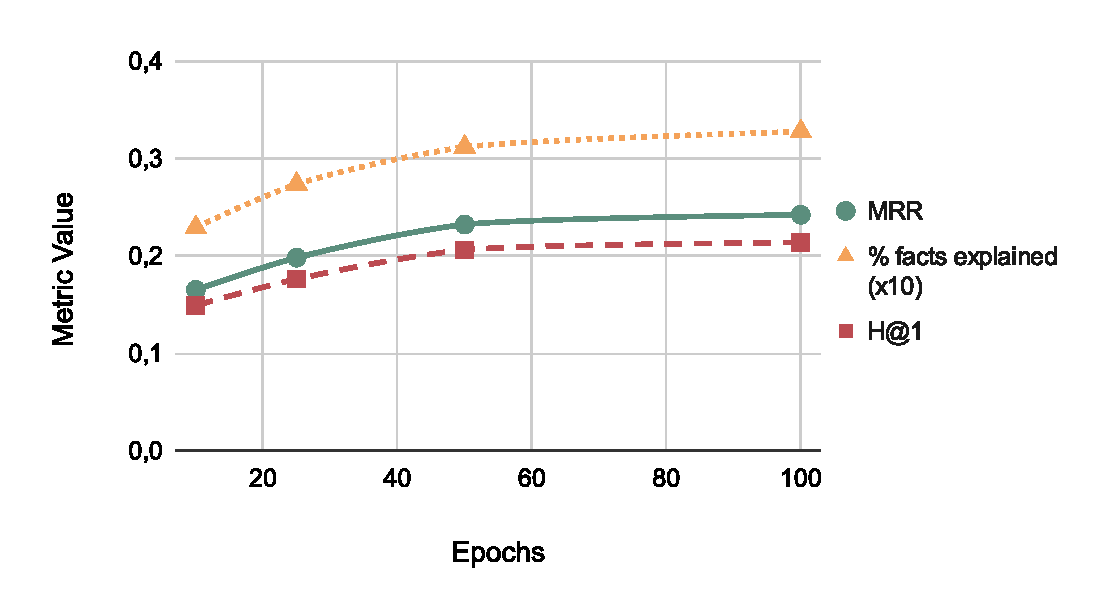
\includegraphics[width=.9\linewidth]{6_kbsextractiondl/figures/coherence_geni_epochs.eps}
    \caption{MRR,Hits@1 and proportion of facts explained for DistMult on DBpedia50 when training for 10, 25, 50 and 100 epochs.}
    \label{fig:coherence_geni_epochs}
\end{figure}

After each model instance is trained, its Mean Reciprocal Rank (MRR) and Hits at 1 (H@1) are computed. Then, the set of object predictions $\mathcal{P}$, alongside with the generated embeddings, is fed into the GEnI framework, which tries to generate a feasible explanation for each prediction $p \in \mathcal{P}$.

This evaluation does not consider the quality or the reliability of the insights, but the proportion of generated explainations with respect to the total amount of facts. Figure \ref{fig:coherence_geni_epochs} depicts the MRR, H@1 and ratio of explained test facts when training DistMult for 10, 25, 50 and 100 epochs.

In addition to the prior evaluation, a second scenario is considered. As stated in Section \ref{6_sec:subsec:geni}, choosing an accurate threshold value is crucial for insight generation. From a coherence standpoint, the threshold value should be inversely proportional to the number of detected rules and correlations, but directly proportional to their reliability. 

In Figure \ref{fig:coherence_geni_epochs}, the threshold value remained constant while the number of epochs increased. The reverse approach is applied in this second scenario: a KGE model trained on 100 epochs remains static throughout the iterations, while the threshold value increases from 0.5 to 0.9 at 0.1 steps. Since the threshold only applies to rule-based and correlation insights, a dataset where these insights are present is needed. FB15k is selected for this scenario. FB15k-237, the refined version of FB15k, is not considered as it removes redundancies and dependencies between triples, which are crucial for rule and correlation extraction. A different KGE model, TransE, is selected to further assess the adaptability of the proposal. Figure \ref{fig:coherence_geni_th} depicts the results of this evaluation, plotting the number of rules and influential facts throughout the different threshold values.

\begin{figure}[t]
    \centering
    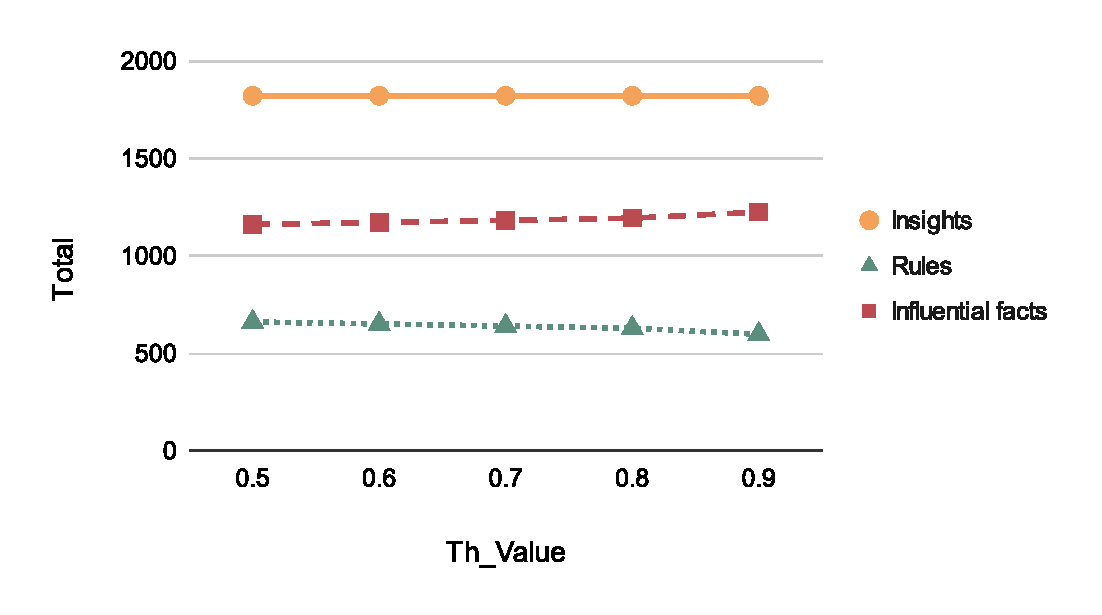
\includegraphics[width=.9\linewidth]{6_kbsextractiondl/figures/coherence_geni_th.eps}
    \caption{Comparison between the number of rules and influential facts per threshold on FB15k on TransE.}
    \label{fig:coherence_geni_th}
\end{figure}

\subsubsection{Meaningfulness Evaluation}
While coherence is quantitative, meaningfulness is qualitative. Therefore, accurately measuring meaningfulness is much more complex, as it requires human understanding. The goal of this evaluation is to assess whether the outputs provided by the framework are readable and coherent from a semantic standpoint while also being compliant with the KG data.

This experimentation stage requires a dataset composed by human-readable elements. FB15k-237 is selected. The triples contained in this dataset refer to real-world entities such as people, places, sports teams, etc. Therefore, it is a fitting choice for this task, as all extracted insights can be easily understood and validated by humans.

In this second stage, TransH is selected. The model is then trained for 100 epochs on the FB15k-237 dataset, generating a set of relation and entity embeddings and a set of object predictions $\mathcal{P}$. For the test set to be manageable, the dataset is divided into training, validation, and test sets with the following proportions:

  \begin{minipage}{\linewidth}
  \begin{align}
   test\_ratio=1000/total\_samples, \nonumber  \\
   val\_ratio=10*test\_ratio, \nonumber \\
   train\_ratio=total\_samples-(test\_ratio+val\_ratio).
\end{align}
\label{eq:split_ratio}
  \end{minipage}

Using these ratios to partition the dataset ensures that the test set comprises 1000 samples, an appropriate and manageable size for manual revision. The set of predictions $\mathcal{P}$, alongside with the relation and entity embeddings are input into the GEnI framework, which attempts to generate a feasible explanation for each prediction $p \in \mathcal{P}$. The same threshold value, 0.75, is employed. This second experimentation stage does not consider the number of explained facts, as the focus is on the quality of the explanations.

\begin{lstlisting}[captionpos=t, float=tp,floatplacement=tbp, breaklines=true, caption=Example of the output produced by the GEnI framework., label=lst:geni_output,basicstyle=\ttfamily,frame=single]
-->Current fact: (/m/026ldz7,/american_football/football_team/current_roster./sports/sports_team_roster/position,/m/01r3hr)
[Success!] Your fact can be inferred using the rule chain (/m/026ldz7, /american_football/football_team/current_roster./sports/sports_team_roster/position, /m/02g_6j) ^ (/m/02g_6j, /sports/sports_position/players./american_football/football_historical_roster_position/position_s, /m/01r3hr) -> (/m/026ldz7,/american_football/football_team/current_roster./sports/sports_team_roster/position,/m/01r3hr)
\end{lstlisting}

GEnI produces human-readable outputs, as showcased in Listing \ref{lst:geni_output}. Nonetheless, just a sample output is not sufficient to assess whether the outcome is meaningful. Meaningfulness relates both human understability and coherence between the output insights and the existing data. 

After the experimentation, GEnI successfully processed 200 predictions out of the total 1000. Each explanation is manually revised according to the following two indications:
\begin{itemize}
    \item I1: All facts related to prediction $p$ share at least one entry with $p$.
    \item I2: All relations featured in the insights must be connected to the predicate in $p$ from a semantic standpoint. Tuples like \textit{(singer, producer)} or \textit{(film, actor)} are examples of this.
\end{itemize}

After the manual evaluation, all explained predictions are compliant with the first indication. For I2, a total of 188 out of the total 200 meet the indication. From the remaining 12 predictions, some remarkable insights can be extracted. For example, two of the predictions of facts \textit{(X,nationality,Y)} are based on the rule chain: 

\begin{align}
    (X, nationality, Y) \leftarrow (X, acted\_in, Z) \wedge (Z, film\_country, Y). 
\end{align}


Although this rule chain is not compliant with the second indicator, it reflects the inference process of the KGE model, evidencing this underlying correlation. 

\subsubsection{Reliability Evaluation}
The final evaluation stage measures the precision and reliability of the framework. Two models are evaluated in this stage: DistMult and TransH. Moreover, two different datasets are considered to provide a wider overview on the performance of the framework. WN18RR is selected to evaluate the performance of DistMult in this task. WN18RR provides a filtered version of the baseline dataset WN18, which encodes facts extracted from the WordNet knowledge graph. As the performance of TransH on WN18RR is subpar and therefore the number of generated insights is minimal, this dataset is replaced by DBpedia50. In this evaluation, both subject and object predictions are computed to generate the set of predictions $\mathcal{P}$. These predictions are processed by the framework generating a set of explanations $\mathcal{X}$. 

The following steps are followed for each KGE model to determine whether the insights and explanations $\mathcal{X}$ computed by GEnI accurately reflect the inference process. First, the facts $\mathcal{F}'$ involved in the explanation of a given prediction $p \in \mathcal{P}$ are removed from the training set. Secondly, the KGE model is retrained from scratch without the facts in $\mathcal{F}'$. A new prediction $p'$ is generated from the original fact on the ablated version of the KGE model. 

There are two possibilities at this stage: $p'= p$ or $p' \neq p$. The first case implies that the facts highlighted by GEnI for predicting $p$ are not correct, as the model still predicts the same output. Instead, $p' \neq p$ is a positive indicator that the insights and explanations provided by GEnI are accurate and reliable. 

\begin{table}[t]
\resizebox{.8\linewidth}{!}{
\begin{tabular}{l|c|c|}
\cline{2-3}
                                                     & \textbf{DistMult on WN18RR} & \textbf{TransH on DBpedia50} \\ \hline
\multicolumn{1}{|l|}{Threshold Value}                & 0.6                         & 0.75   \\
\multicolumn{1}{|l|}{MRR}                & 0.31                         & 0.16   \\
\multicolumn{1}{|l|}{H@1}                & 0.28                         & 0.11   \\
\hline
\multicolumn{1}{|l|}{\# Explained Facts}             & 191                         & 1927                         \\
\multicolumn{1}{|l|}{\# Facts Changing Prediction}   & 145                         & 1272                         \\
\multicolumn{1}{|l|}{\textbf{Reliability Coefficient}} & \textbf{0,76}               & \textbf{0,66}                \\ \hline
\multicolumn{1}{|l|}{\# Rules Detected}              & 0                           & 12                           \\
\multicolumn{1}{|l|}{\# Correlations Detected}       & 0                           & 0                            \\
\multicolumn{1}{|l|}{\# Influential Facts Detected}  & 191                         & 1993                         \\ \hline
\end{tabular}
}
\caption{Reliability results on DistMult on WN18RR and TransH on DBpedia50. The number of rules, correlations, and influential facts per experiment are also reported.}\label{tab:reliability_results}
\end{table}

Hyperparameters for this experimentation are selected focusing on resource optimization instead of performance due to the elevated resource and time consumption required for this evaluation. Instead of generating embeddings of dimension 200 and training for 200 epochs, both the dimension and the epochs are reduced to 100. The threshold is set to 0.6 for WN18RR due to the increased difficulty of this dataset. A threshold value of 0.75 is used for DBpedia50. 

Table \ref{tab:reliability_results} reports the results obtained from the two experimentation setups. The reliability coefficient is computed as the number of facts changing their prediction value when their associated insights facts are removed in the training set by the total amount of facts explained.

\subsection{Result Analysis}\label{6_sec:subsec:geni_results}
In the coherence evaluation, a KGE model was trained using the same dataset for an increasing number of epochs to assess the impact that the performance of the KGE model has on GEnI. Figure \ref{fig:coherence_geni_epochs} shows that there exists a direct correlation between these two elements. Moreover, it shows how the curvature of the plots for the percentage of facts explained (triangle points, dotted line), and the H@1 (square points, dashed line) fit almost perfectly. Aside from evidencing the correlation between the performance of the KGE model and the framework, this experimentation also showcases the existing difficulties when generating insights for predictions.

The KGE model remains stable during the second coherence evaluation, using the same model instance for all experimentation iterations. The input threshold is the variable in this scenario, increasing its value throughout the experimentation. From a coherence standpoint, the lower the threshold is, the more rules and correlations should be generated. However, the threshold should not impact the total number of generated insights, as phase three of the framework is not bounded to this value. Therefore, if a rule can be used to explain a prediction, the same prediction can also be explained based on a set of influential facts. Figure \ref{fig:coherence_geni_th} shows how GEnI successfully handles this issue. The number of detected rules decreases proportionally with the increment of the threshold value. While 660 predictions could be successfully explained using rules with a threshold value of 0.5, this number steadily decreases to 597 when the threshold rises to 0.9. Nonetheless, this does not affect the total number of insights (circle points, continuous line), which stays static throughout the different threshold values. Therefore, GEnI compensates for the decrease in the number of computed rules by increasing the number of predictions explained by influential facts, subsequently maintaining the performance of the framework. 

Regarding meaningfulness, the evaluation confirms that the output generated by GEnI is readable, understandable from a human perspective, and coherent with the KG and the model output. It also evidences that GEnI output can highlight existing biases within the KGE, even if the output is not coherent from a semantic standpoint.

Two opposite scenarios were studied regarding reliability: DistMult on WN18RR and TransH on DBpedia50. Table \ref{tab:reliability_results} reports the results obtained. In DistMult, all insights were obtained during the third phase of the framework. As WN18RR does not include inverse triples or redundancies, it is coherent with the obtained output, where predictions are explained by their most influential facts. From a total of 191 explained predictions, 145 experienced a change in their prediction after removing those training facts detected as influential by GEnI. This result equates to a reliability coefficient of 76\%.

A different behavior is exhibited on the evaluation of TransH on DBpedia50. One of the main differences between both scenarios is the number of explained predictions, which is about ten times higher in this scenario. This result may be directly related to the complexity of the dataset. Another remarkable difference is the performance of each KGE model, which is slightly better in DistMult with respect to TransH.

The reliability coefficient achieved by TransH on DBpedia50 is slightly lower, scoring a 66\% of predictions changed after retraining. This result can be due to: i) the total amount of explained facts, and ii) the performance of each KGE model. While DistMult scored a MRR of 0.31, TransH only reached a 0.16, which denotes a lesser expressivity of the embeddings. Although it may not be sufficient to establish a relation between the performance of the KGe and the reliability of GEnI, it is an indicator that improving the performance of the KGE model could directly reflect into the results achieved by GEnI.


\subsection{Design Compliance}\label{6_sec:subsec:geni_design_compliance}
Figure \ref{fig:design_compliance_geni} portrays the design parameters of the GEnI, the proposed explainability framework for KGE predictions: 
\begin{figure}[t]
    \centering
    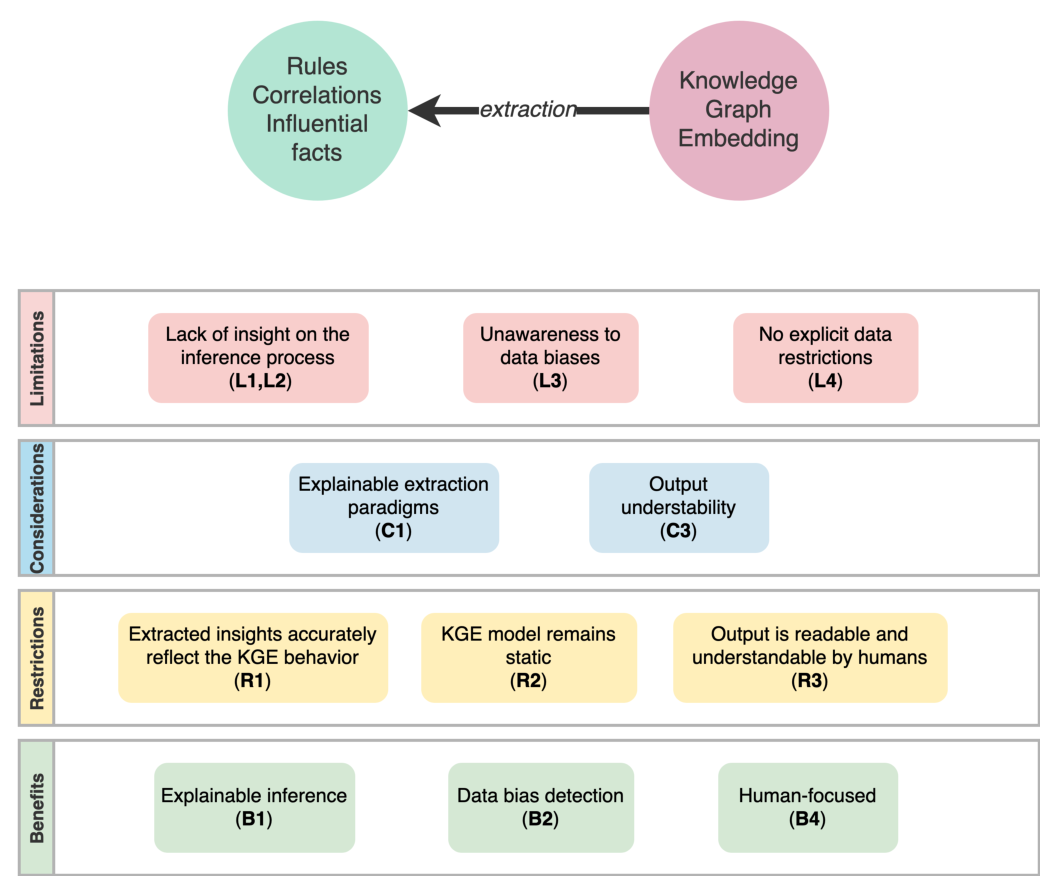
\includegraphics[width=\linewidth]{6_kbsextractiondl/figures/Instance_GENI_extraction_DL.eps}
    \caption{Overview on the design parameters of insight extraction on KGE models. In bold, the general parameters as depicted in \ref{fig:kbs_extra_dl_overview}.}
    \label{fig:design_compliance_geni}
\end{figure}

\subsubsection*{Limitations}
\begin{itemize}
    \item \textbf{Lack of insight on the inference process.} Most KGE models are opaque by design (\ref{kbsextradl_L_opacity}). When the model makes a prediction, only the output and the fact probabilities are known. This information may serve as a reference to extract some conclusions about the inference process. However, the effort of understanding the behavior of the model and the inference process is done by the user, and not by the model itself (\ref{kbsextradl_L_human}).
    
    \item \textbf{Oblivious to data biases.} KGE models learn from data, which is subject to biases. Moreover, the presence of biases in the data can lead to the generation of misleading inference patterns. Additionally, it can lead to inference patterns that, while accurate, may not be coherent. One example of such biases is the prediction of the profession $nurse$ for those entities that are denoted to have a $female$ genre. (\ref{kbsextradl_L_ethical}). 
    
    \item \textbf{No explicit data restrictions.} Section \ref{4_sec:ontointro_kgc} outlined this issue within KGE models. As inference patterns are learned directly from the data, only soft restrictions are inferred. Besides hindering its transferability (\ref{kbsextradl_L_transferability}), the lack of explicit restrictions about the data difficults the understanding of the inference process.
\end{itemize}

\subsubsection*{Considerations}
\begin{itemize}
    \item \textbf{Explainable extraction paradigms.} The final goal of the proposal is to accurately explain the inference process of KGE models. Therefore, symbolic paradigms should be used to extract information from the KGE, such that the subsymbollic information encoded in the model is translated into an understandable, human-readable output (\ref{kbsextradl_C_paradigm}). 
    
    \item \textbf{Output understandability.} The selected extraction models are symbolic and can therefore be read by humans. The raw extracted insights, while readable, may not be understood by non-expert users (\ref{kbsextradl_C_user}). Therefore, the output must be reformulated in a non-expert mode such that it can be understood by humans.
\end{itemize}

\subsubsection*{Restrictions}
\begin{itemize}
    \item \textbf{Extracted insights accurately reflect the KGE behavior.} One of the key challenges of explainability approaches is reliability. This is an essential aspect of the proposed framework, where insights are mined from the embeddings and not the data to accurately reflect the behavior of the model. Moreover, the performance of the proposed framework is directly proportional to the performance of the KGE model, as evidenced by the experimentation results (\ref{kbsextradl_R_behavior}). 
    
    \item \textbf{KGE model remains static.} The KGE model is the element to explain. For the extracted insights and explanations to accurately reflect the model behavior, it is essential that the KGE model remains unchanged during the process. If the KGE model changes, then the extracted insights may turn inaccurate (\ref{kbsextradl_R_performance}). 
    
    \item \textbf{Output is readable and understandable by humans.} Symbolic models are inherently readable. Understandability induces an additional level regarding readability, where the output not only must be presented in a human-readable format, but accessible and simplified. The output provided by the proposed framework not only is expressed in natural language, but summarizes the most important findings of the explainability process such that they can be easily understood by humans (\ref{kbsextradl_R_human}). 
\end{itemize}

\subsubsection*{Benefits}
\begin{itemize}
    \item \textbf{Explainable inference.} The main and most prominent benefit is the increased understandability of the inference process of the KGE model. While the proposed framework may not be able to fully explain all model predictions (both correct and incorrect), it provides a clear and accurate insight on some of the inferential mechanisms used by the model (\ref{kbsextradl_B_interpretability}).
    
    \item \textbf{Data bias detection.} As previously remarked, KGE models are subject to learning biased inferential patterns. These patterns may lead to inaccurate predictions. Insights on the inference can help finding the potential causes of the bias (\ref{kbsextradl_B_bias}).   
    
    \item \textbf{Human-focused.} Opposite to regular KGE models, the proposed framework considers the user as a central element. Therefore, the user not only impacts the behavior of the system, but the output is also formulated in a readable, human-understandable way (\ref{kbsextradl_B_human}). 
\end{itemize}
%%-----
%\section{Explainability on Knowledge Graph Completion}

%\section{GEnI: A Model-Agnostic Framework for Generating Explanations and Insights on Link Predictions}

%\section{Design Compliance II}
\section{Summary}\label{6_sec:summary}